\section{WS-*协议}

\subsection{WS-*协议的概念}
WS-* 协议是指除了核心标准外地扩展 Web Service 协议。不同公司和不同组织都在不断地提供对 Web Service 的扩展,大致可分类为以下几种:

\vspace{-0.5em}
\begin{table}[H]
    \centering
    \resizebox{\textwidth}{!}{\begin{tabular}{|l|l|}
    \hline
    XML Specification(XML定义)                 & Resource Specifications(对资源进行说明)                            \\ \hline
    Messaging Specification(消息传递)           & \begin{tabular}[c]{@{}l@{}}Web Services Interoperability (WS-I) Specification\\ (说明Web Service可互操作性)\end{tabular} \\ \hline
    Metadata Exchange Specification(元数据交换)   & Transaction Specifications(事务定义)                         \\ \hline
    Security Specification(安全性)            & Management Specifications(管理规范)                          \\ \hline
    Privacy(隐私)                           & Draft Specifications(草案规范)                               \\ \hline
    Reliable Messaging Specifications(可靠消息) & Other(其他)                                              \\ \hline
    \end{tabular}}
\end{table}
\vspace{-1.5em}

\subsection{WS-*协议具体分类}
\begin{figure}[H]
    \vspace{-1em}
	\centering
	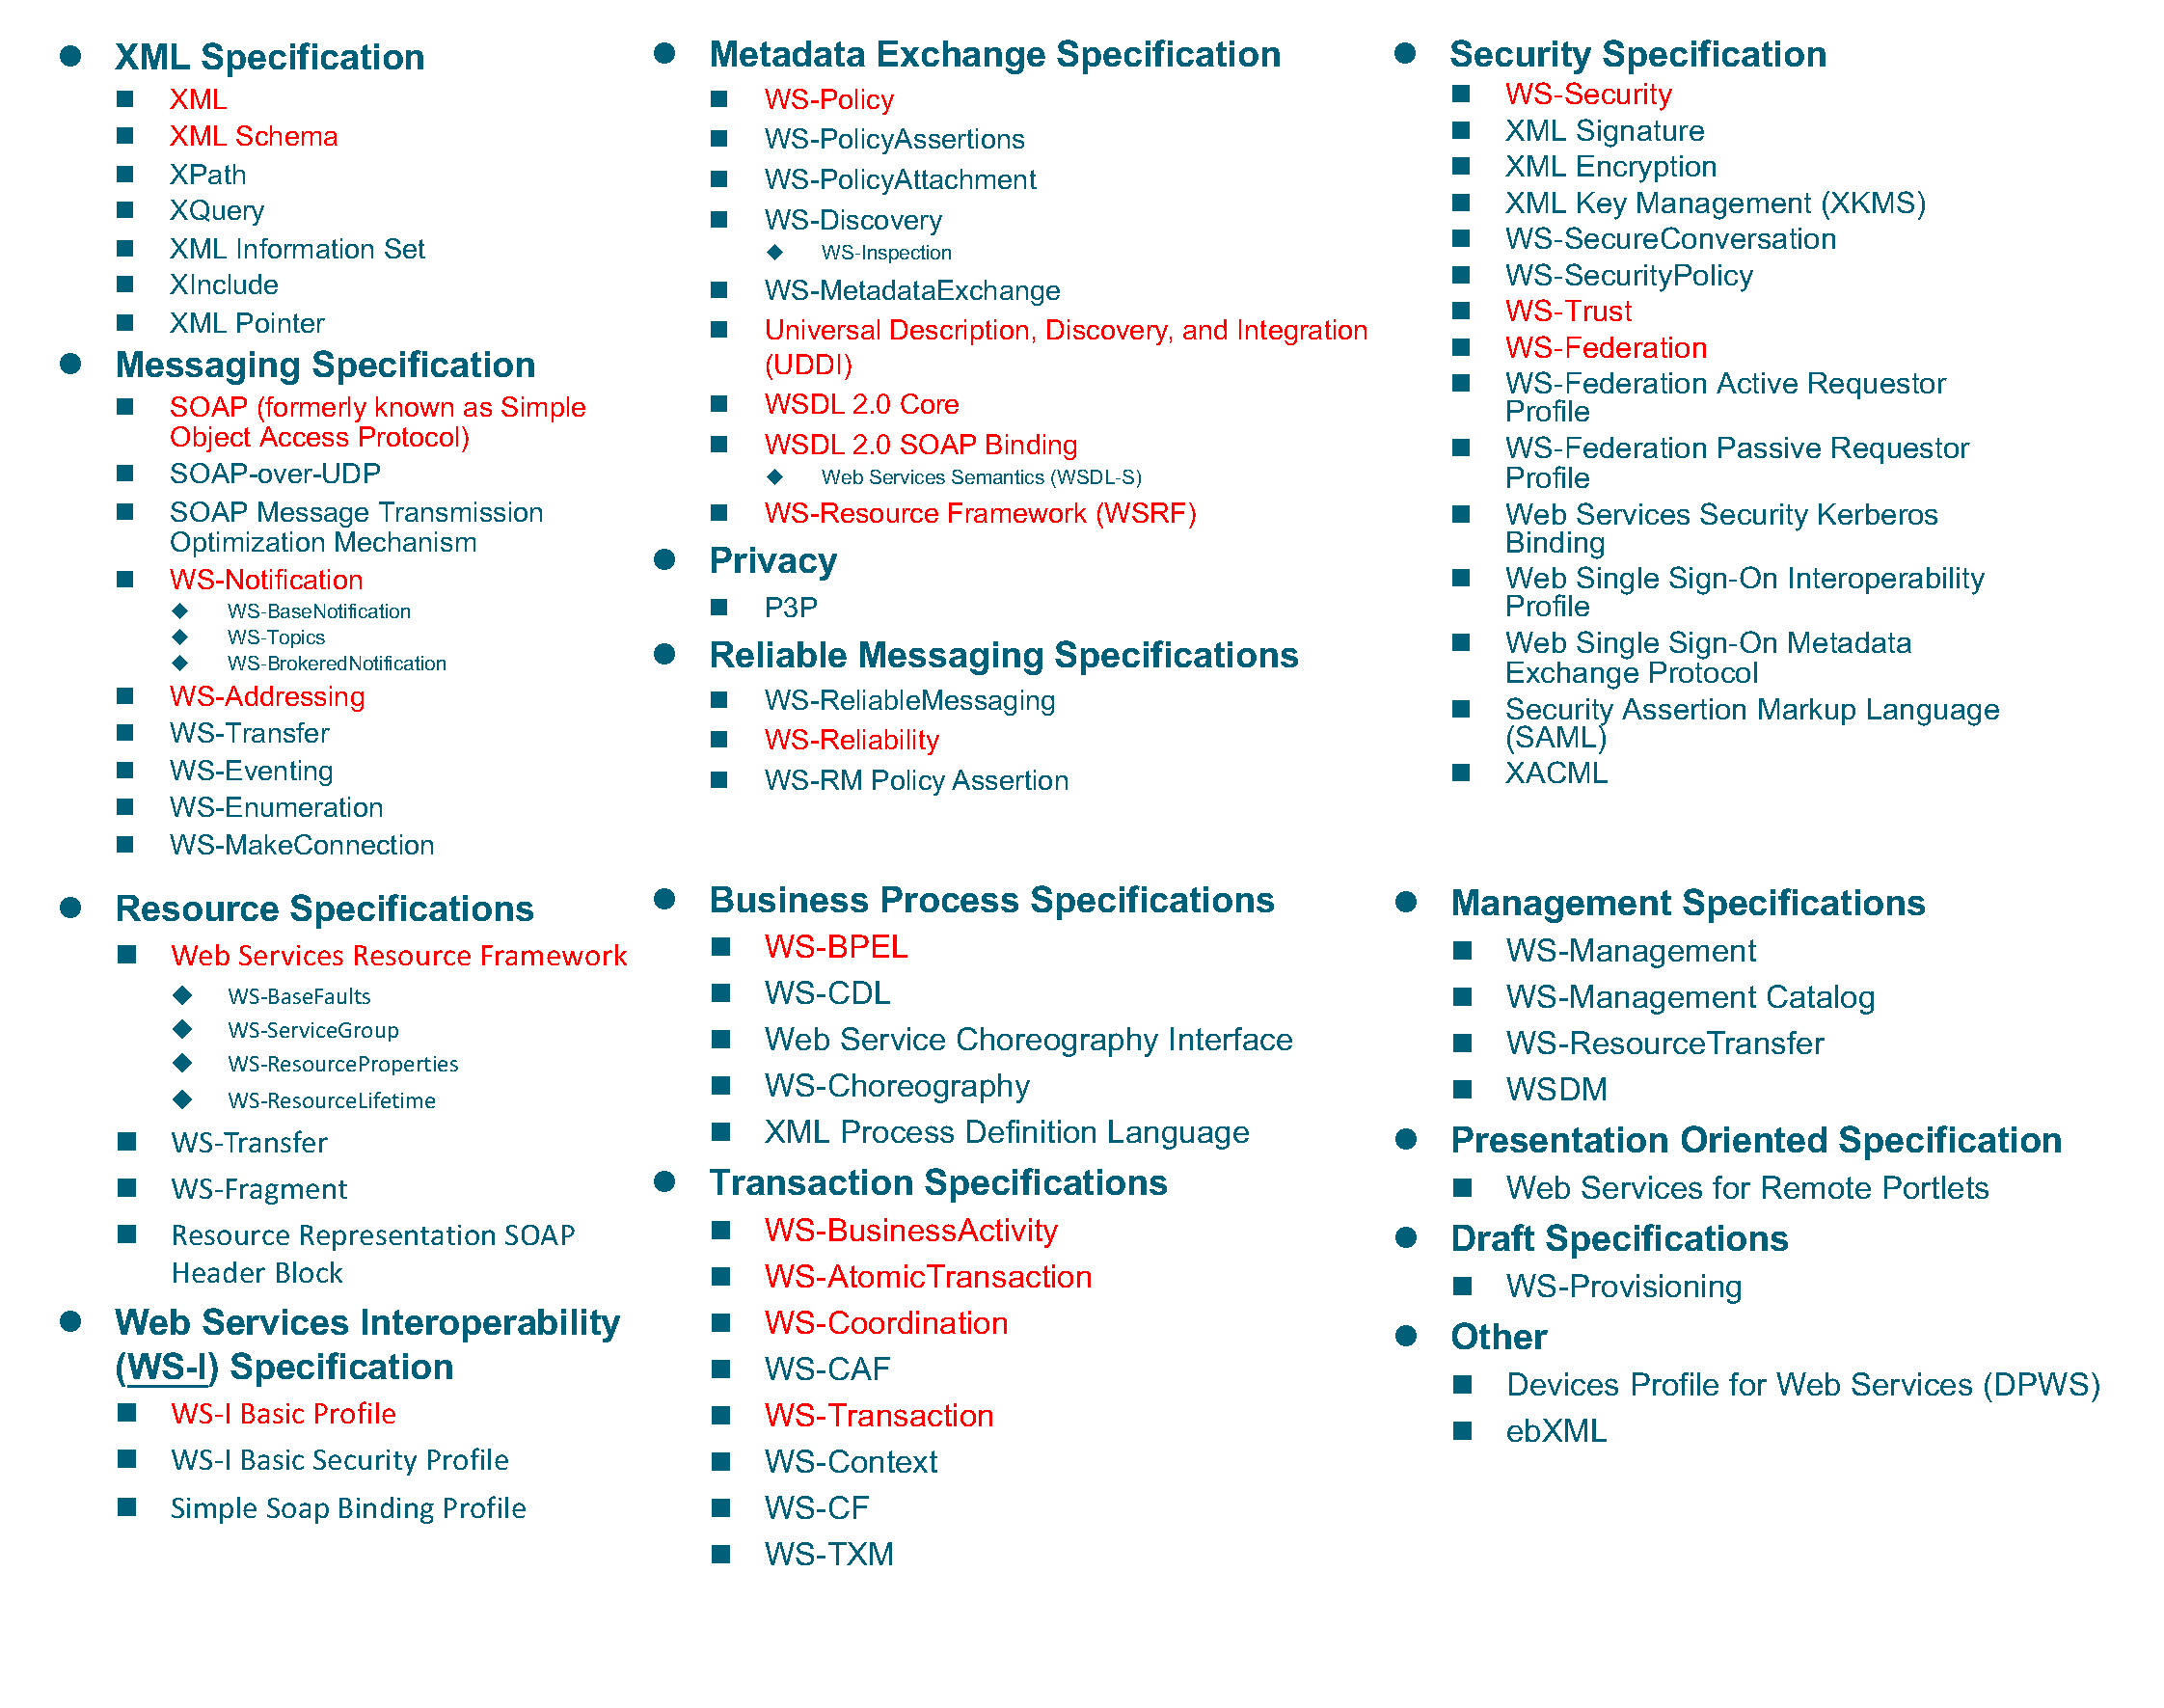
\includegraphics[width=0.97\textwidth]{images/WS-*协议具体分类.pdf}
    \vspace{-1.5em}
\end{figure}

\subsection{WS-Addressing}

\subsubsection{Web Service中的消息分发}
\begin{itemize}
    \item 为了正确处理,消息接收者必须具备识别所需要调用的 Web Service 的能力
    \item 由于在 WSDL 中没有定义,服务提供者在开发服务时,需要自己来区分消息的不同类型
    \begin{itemize}
        \item 在单个地址上部署单个服务时,采用XSD,为不同的服务能力的不同消息说明不同的QNames
        \item 在单个地址上部署多个服务时,必须在全局考虑所有服务中的消息类型
    \end{itemize}
    \item 如服务提供者不能达成上述目标,尤其在使用通配类型(\#any, \#none)时,必须提供消息分发机制
    \item 在带状态的 Web Service 中,也需要消息分发机制,来识别同一个服务的不同实例
\end{itemize}

\subsubsection{WS-Addressing协议}
WS-Addressing规范提供了这样一种消除歧义的机制
\begin{itemize}
    \item 它包括一个可标记为必需的扩展元素,并定义了一个必需的操作属性,其值始终存在于符合要求的消息传递中
    \item 操作属性的值可以用于由接收者消除歧义的消息,并且在WS-Addressing规范中有一种明确定义的方法来将操作与消息相关联
    \item 此外,WS-Addressing还提供了适当的默认操作值,以唯一标识每种消息类型
    \item WS-Addressing定义了端点引用和SOAP头块
\end{itemize}

\paragraph*{使用WS-Addressing的SOAP信息}~{} \par
\begin{figure}[H]
    \vspace{-0.5em}
	\centering
	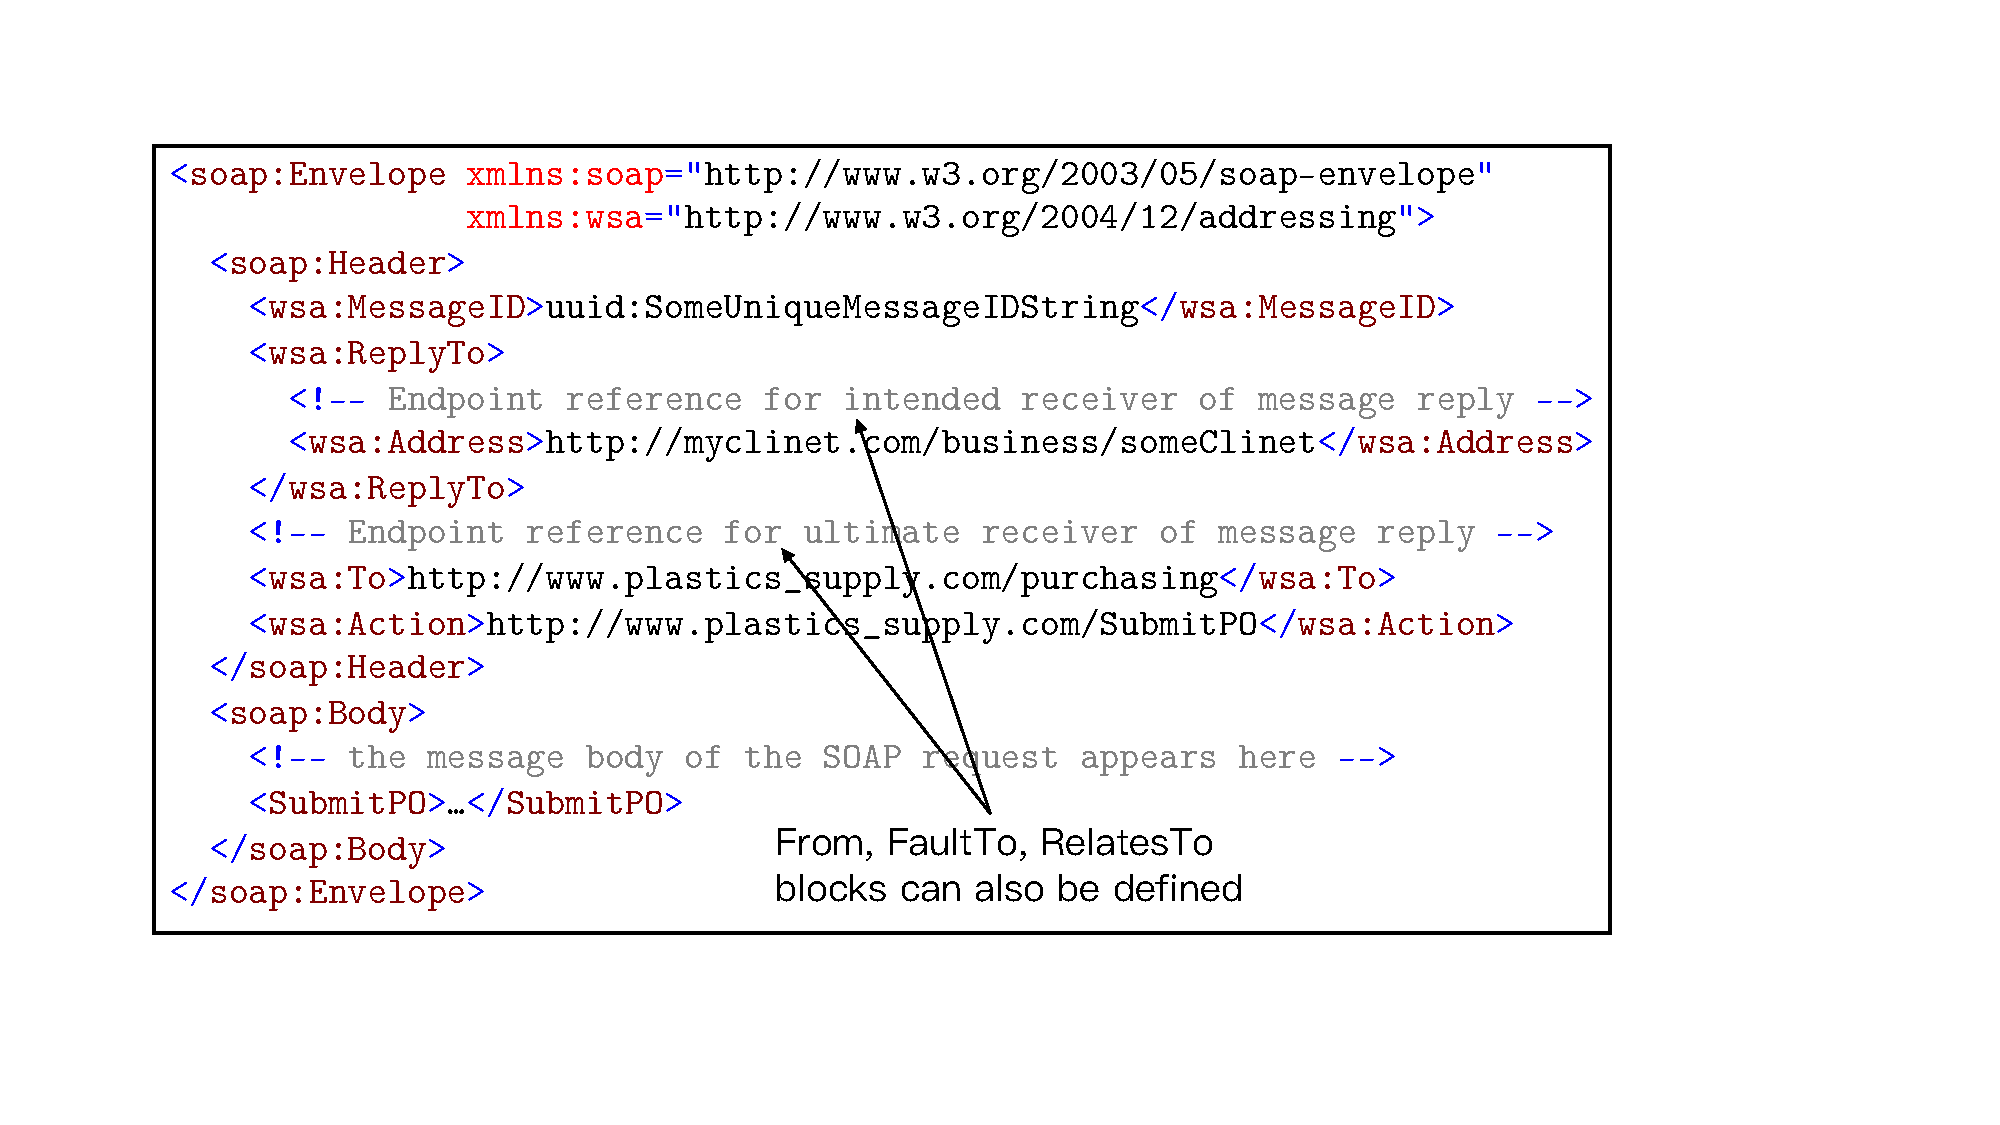
\includegraphics[width=0.8\textwidth]{images/使用WS-Addressing的SOAP信息.pdf}
    \vspace{-1em}
\end{figure}

\paragraph*{端点引用}~{} \par
\begin{figure}[H]
    \vspace{-0.5em}
	\centering
	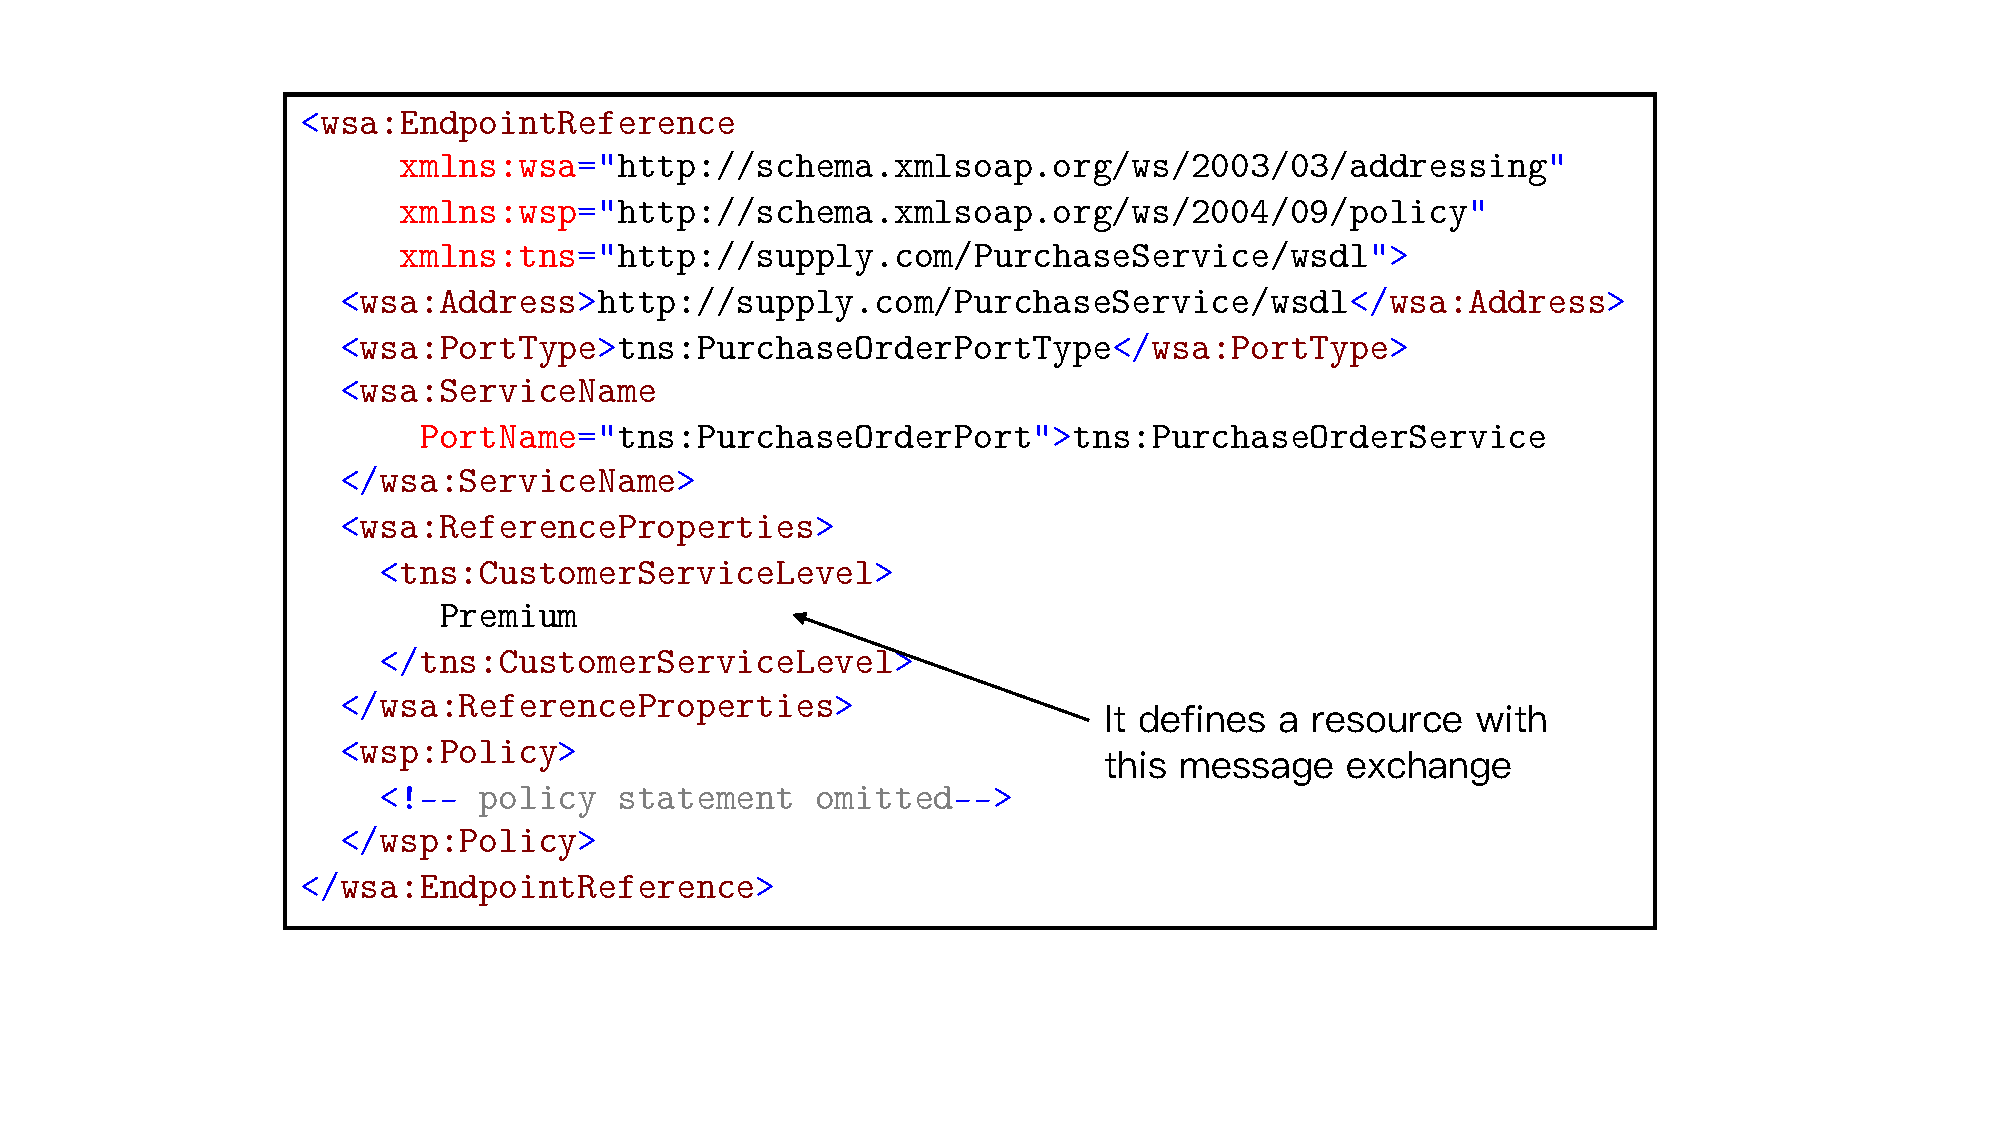
\includegraphics[width=0.7\textwidth]{images/端点引用.pdf}
    \vspace{-1em}
\end{figure}

\begin{figure}[H]
	\setcounter{subfigure}{0}
	\centering
	\vspace{-0.5em}	
	\subfloat[Request Message]{
	\begin{minipage}[t]{0.55\linewidth}
	\centering
	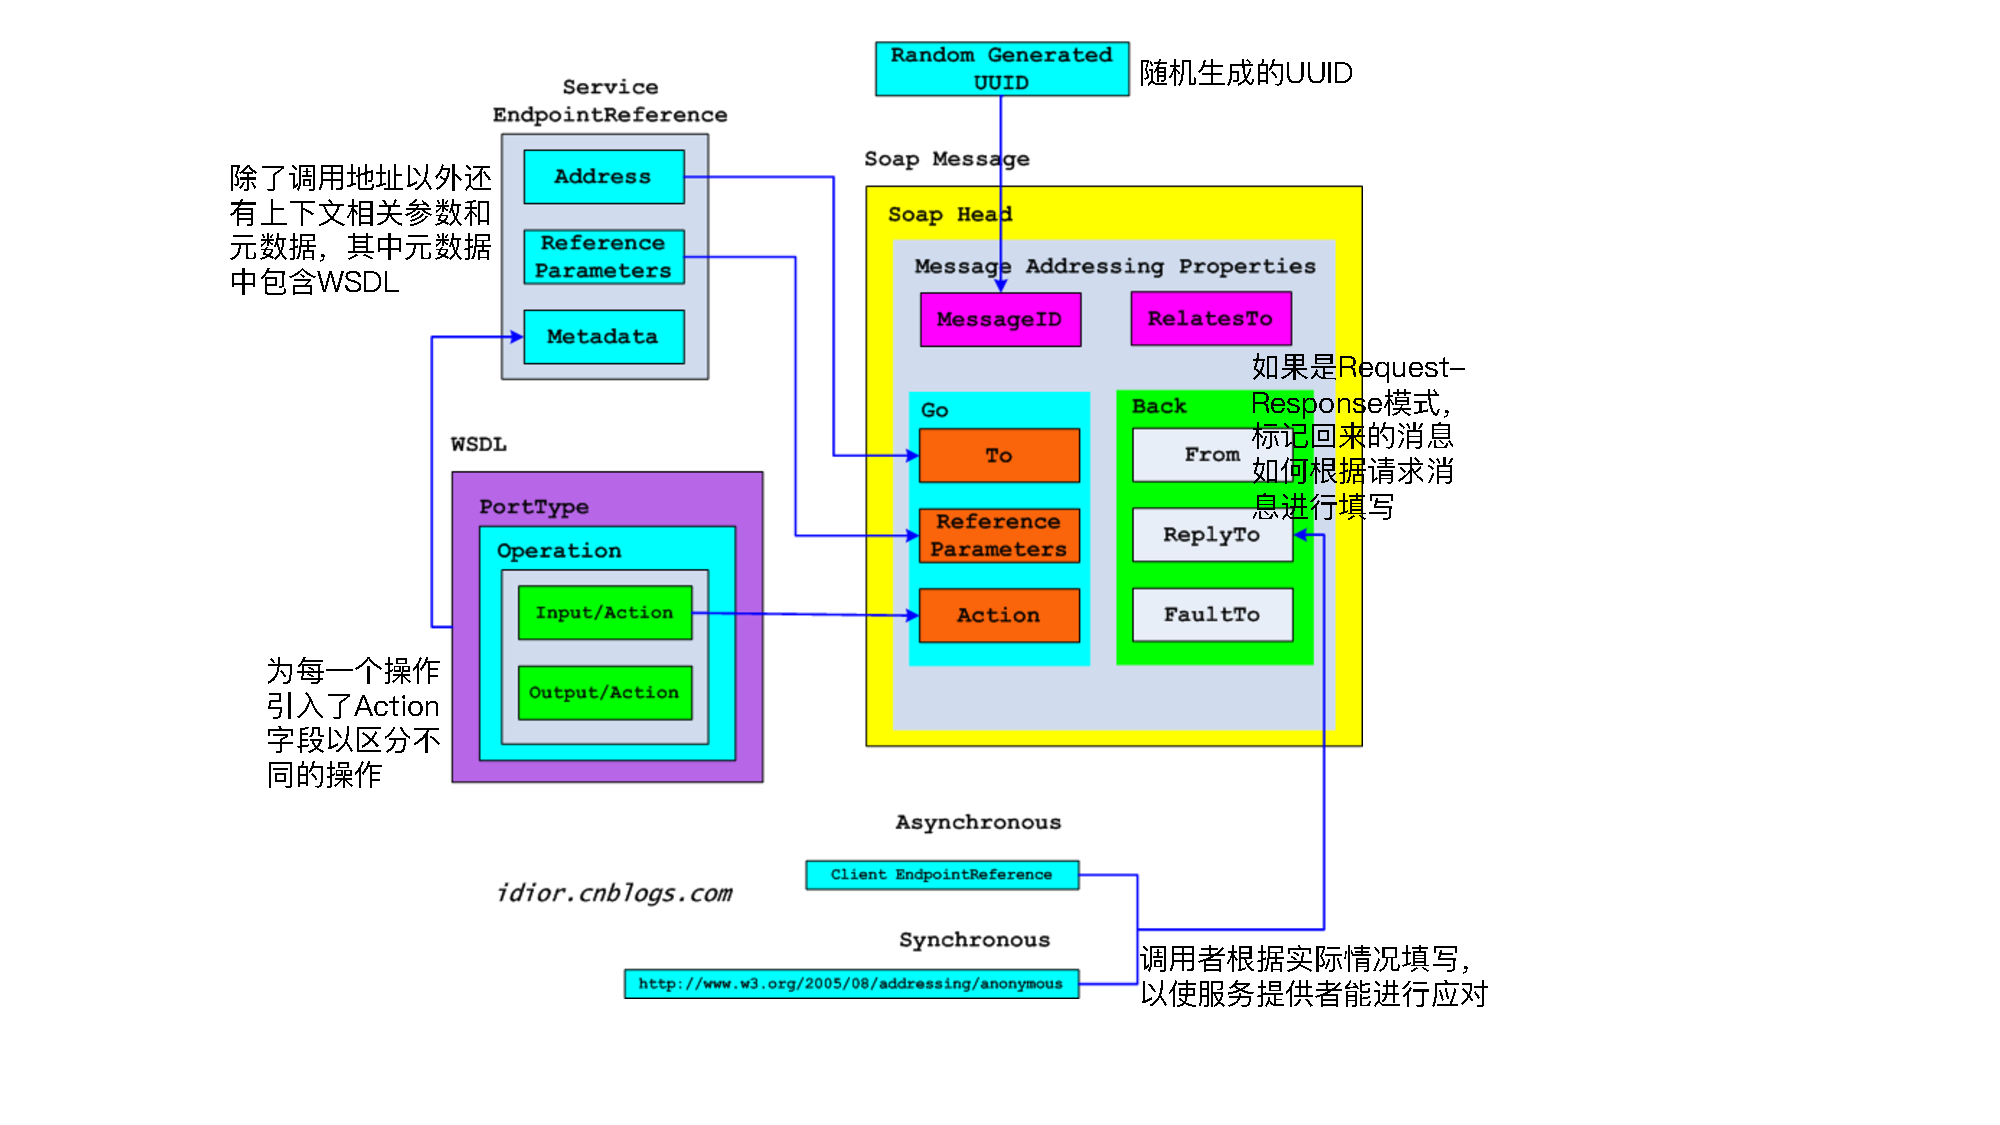
\includegraphics[width=\linewidth]{images/Request Message.pdf}
	\end{minipage}
	}
	\subfloat[Response Message]{
	\begin{minipage}[t]{0.42\linewidth}
	\centering
	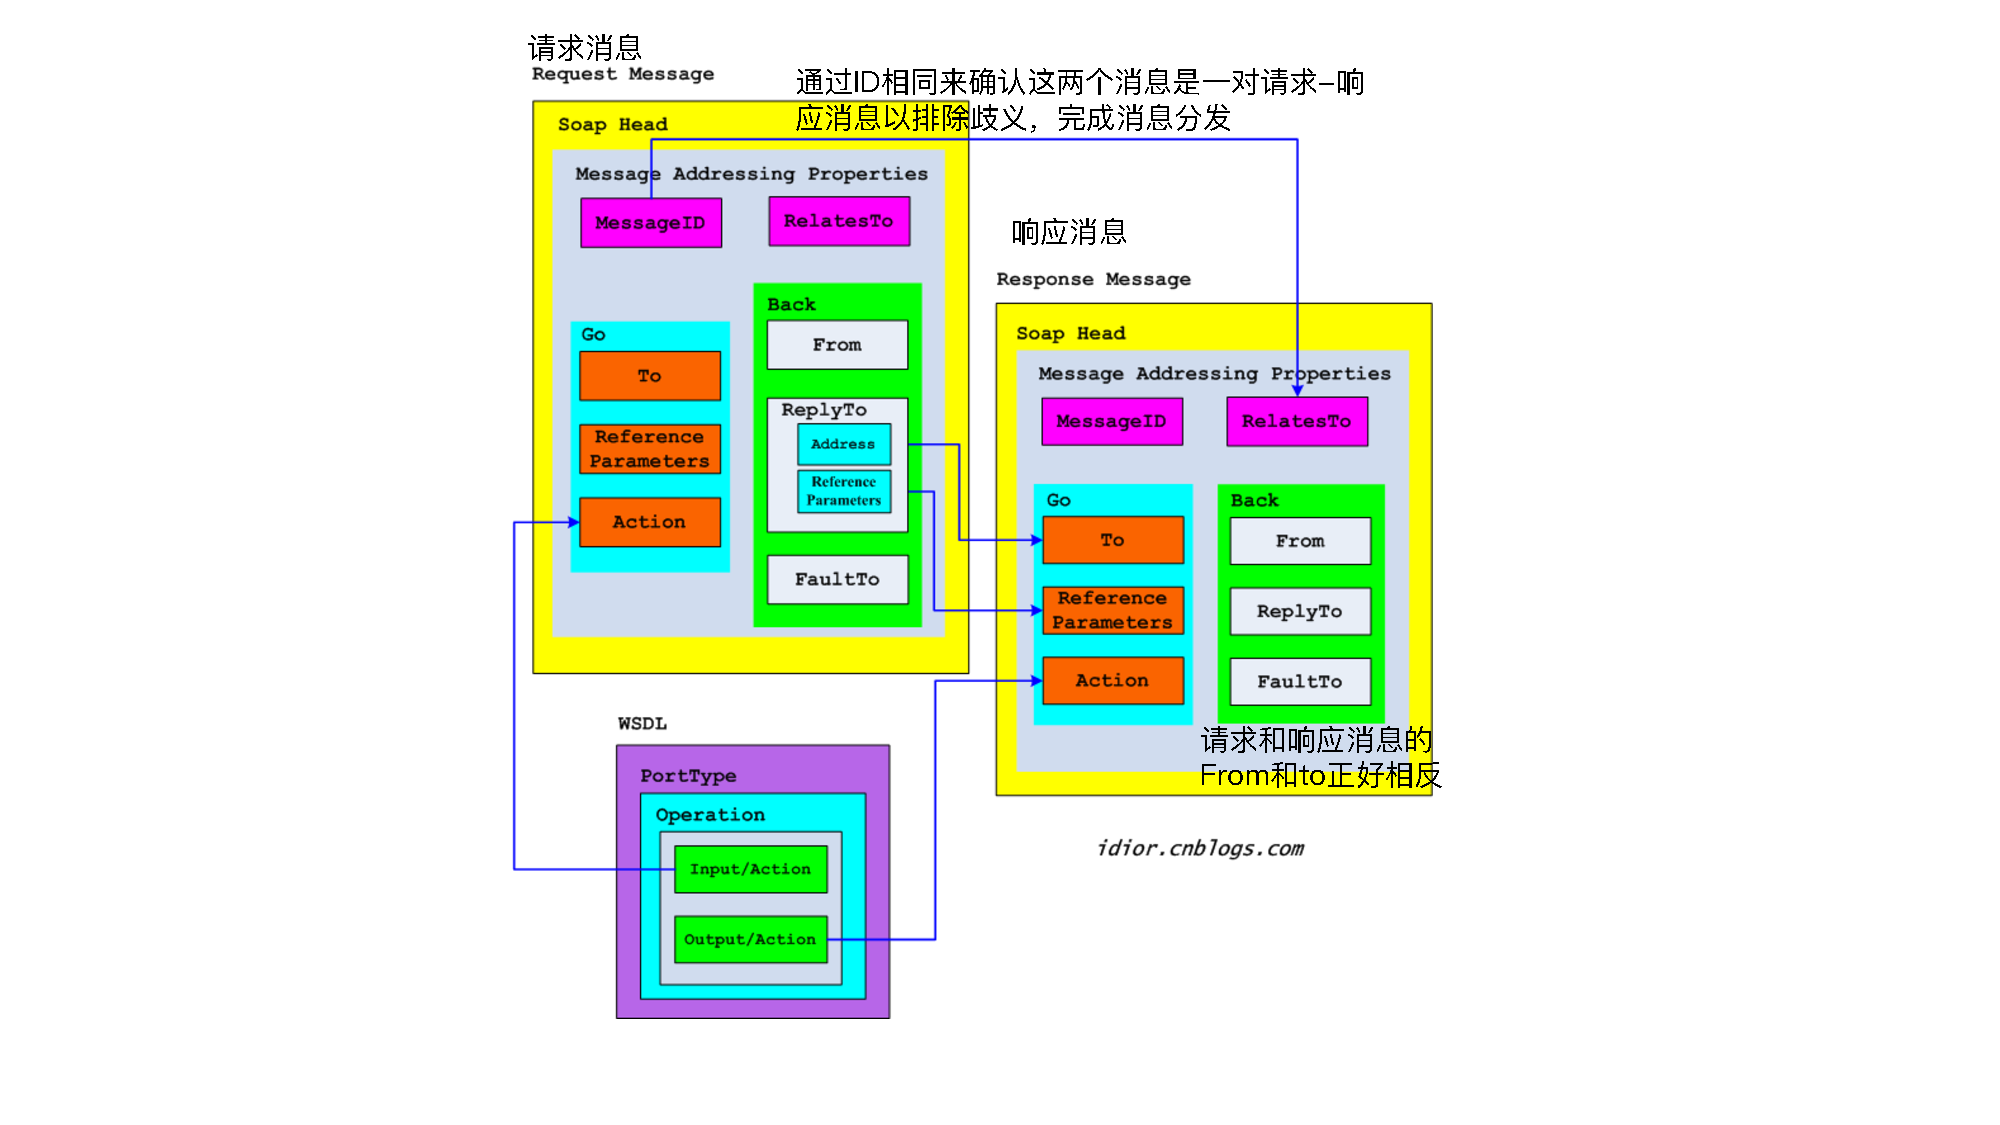
\includegraphics[width=\linewidth]{images/Response Message.pdf}
	\end{minipage}
	}
	\centering
	\vspace{-1em}
\end{figure}

\subsection{WSRF}

\subsubsection{无状态和有状态的Web Service}
\begin{itemize}
    \item 无状态的Web服务不会捕获或维护状态,是没有上下文的Web服务
    \item 有状态的Web服务为各种类型的消费者提供个性化服务,持久化信息以更好地为消费者服务,综合服务需要协作
\end{itemize}

\vspace{-0.5em}
\begin{spacing}{1.2}
    \begin{longtable}{|m{5cm}|m{7cm}|}
    \hline
    \multicolumn{1}{|c|}{\textbf{无状态 Web Service}} & \multicolumn{1}{c|}{\textbf{有状态 Web Service}} \\ \hline
    \vspace{-1.3em}
    \begin{itemize}[leftmargin=1.5em,itemsep=-3pt]
        \item 不获取和维护状态
        \item 无上下文
        \item 可扩展性好,容错性好
        \item 轻量级
    \vspace{-1.5em}
    \end{itemize}                                           
    & 
    \vspace{-1.3em}
    \begin{itemize}[leftmargin=1.5em,itemsep=-3pt]
        \item 为不同消费者服务,且提供个人化服务
        \item 持有状态
        \item 支持需要协作的复杂服务
        \item 需要更多编码和额外的处理资源
        \item 重量级
    \vspace{-1.5em}
    \end{itemize}  
    \\ \hline
\end{longtable}
\end{spacing}
\vspace{-1em}

\begin{figure}[H]
	\setcounter{subfigure}{0}
	\centering
	\vspace{-0.5em}	
	\subfloat[无状态和有状态WebService举例]{
	\begin{minipage}[t]{0.47\linewidth}
	\centering
	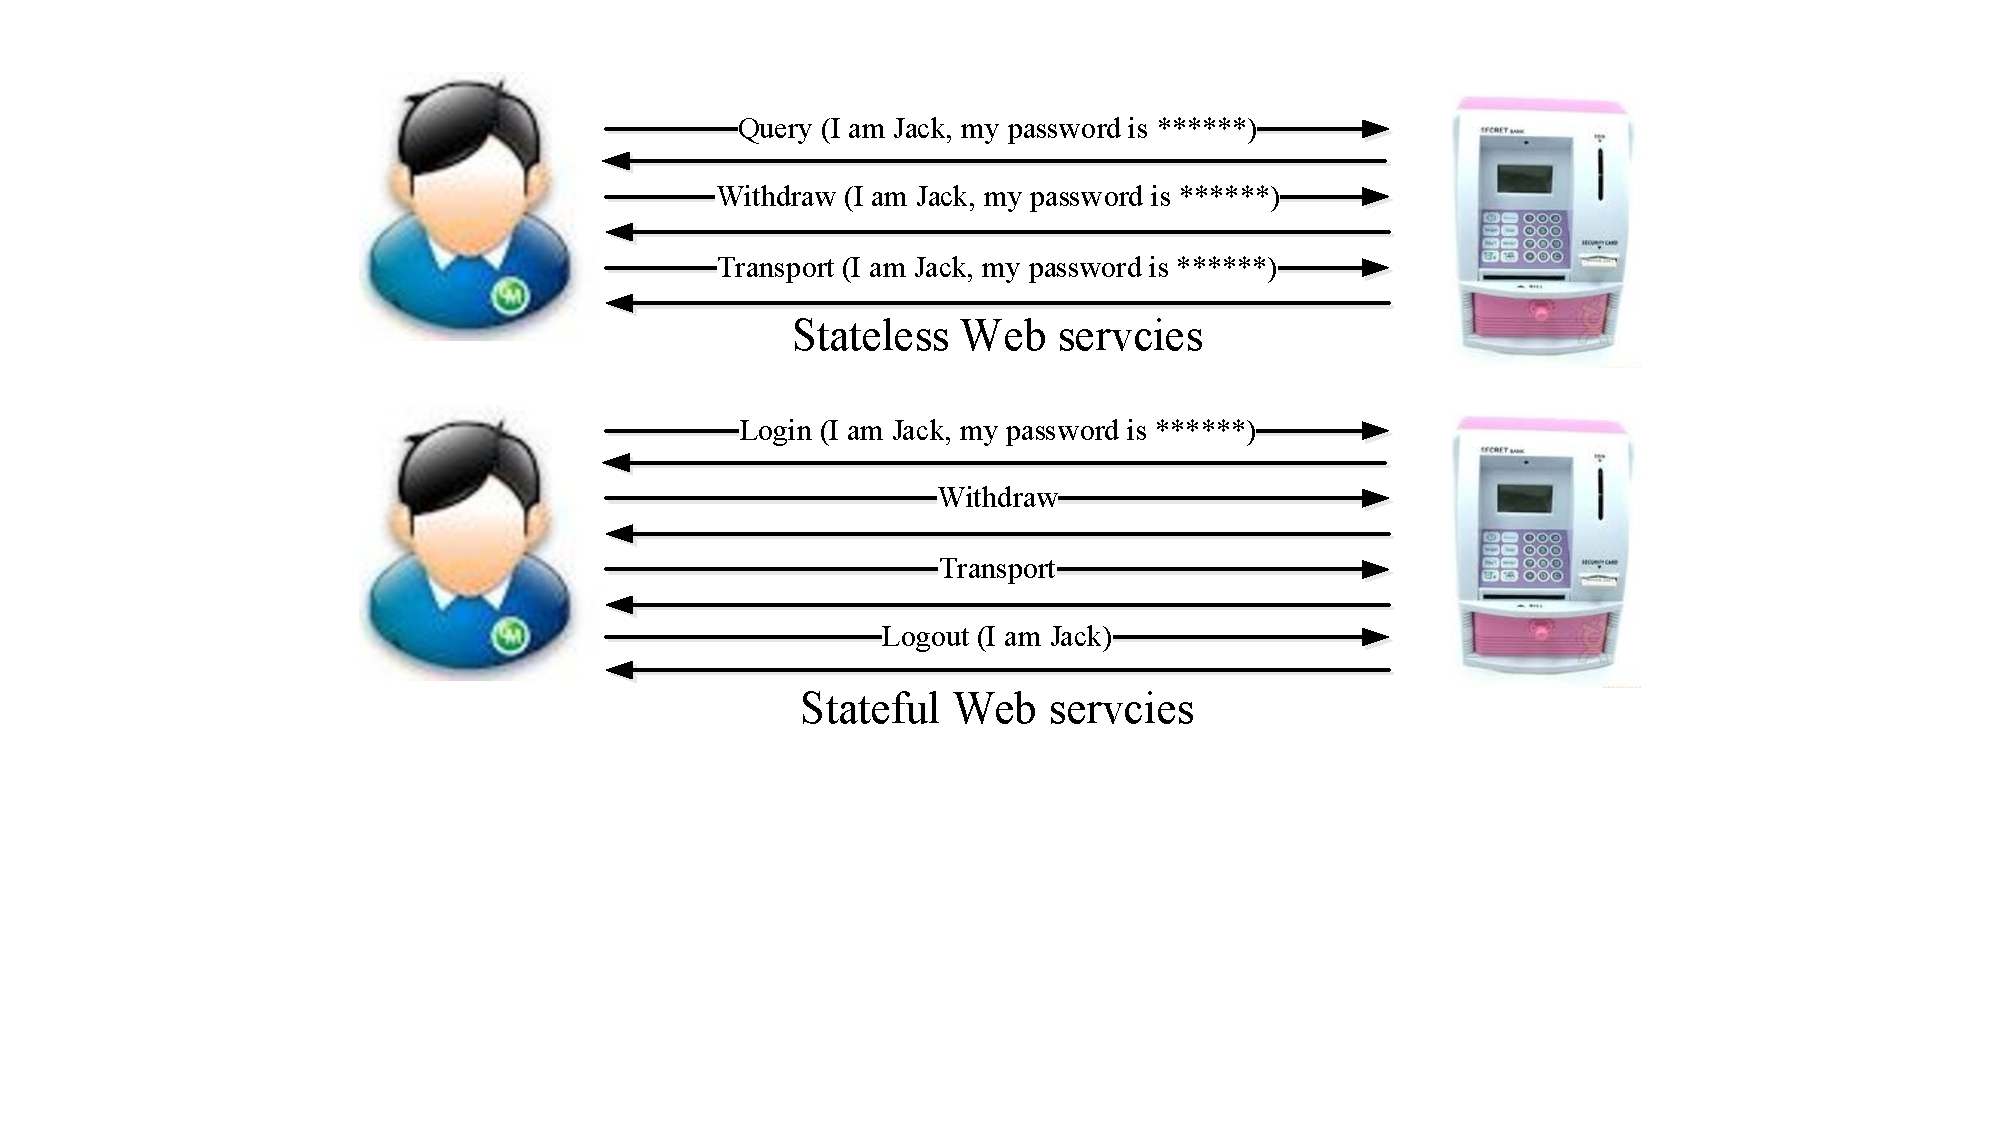
\includegraphics[width=\linewidth]{images/Stateless and Stateful Web services1.pdf}
	\end{minipage}
	}
	\subfloat[对于资源修改需要指明是对哪个资源进行操作的]{
	\begin{minipage}[t]{0.47\linewidth}
	\centering
	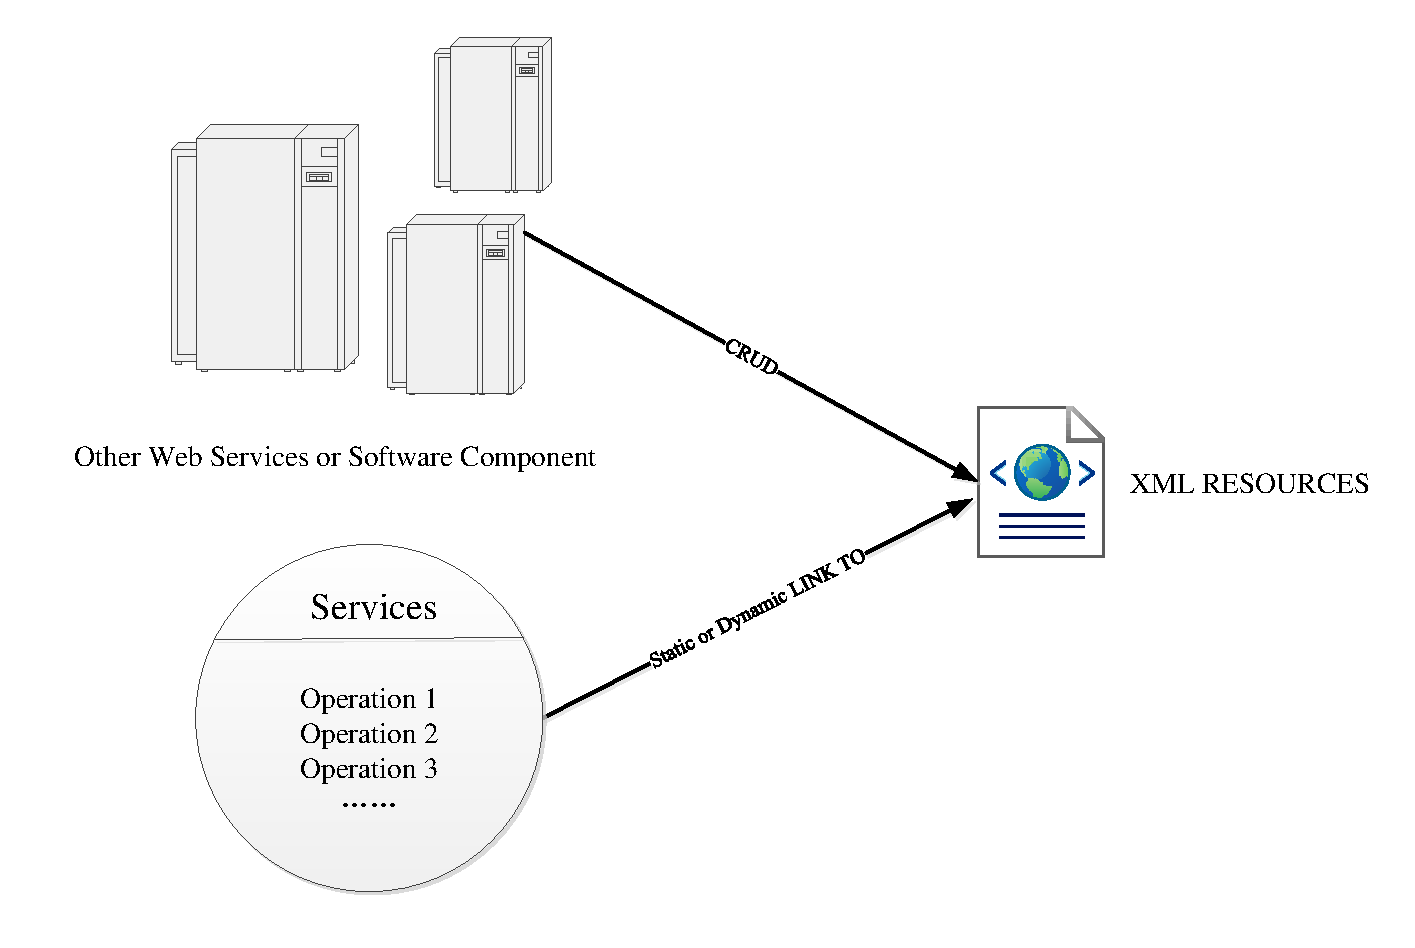
\includegraphics[width=\linewidth]{images/Stateless and Stateful Web services2.pdf}
	\end{minipage}
	}
	\centering
	\vspace{-1em}
\end{figure}

\subsubsection{Web Service 资源框架(WSRF)}
WSRF(Web Services Resource Framework, Web Service资源框架)定义了一套规范体系,用于使用Web服务管理和访问有状态资源。它包含四个规范集,通过Web服务接口访问资源的内部状态:
\begin{itemize}
    \item WS-ResourceProperties (WS-RP):定义如何访问和管理资源的属性(例如,资源名称、创建时间、所有者等)
    \item WS-ResourceLifetime (WS-RL):定义如何管理资源的生命周期,包括创建、销毁、暂停和恢复
    \item WS-BaseFault (WS-BF):定义一种标准的故障报告格式,用于在发生错误时向服务消费者传递错误信息
    \item WS-ServiceGroup (WS-SG):定义如何管理和操作一组相关的服务
\end{itemize}

WSRF支持资源属性的动态创建和支持资源的销毁(立刻销毁与基于时间的计划销毁)

\paragraph*{状态资源的定义}~{} \par
\begin{figure}[H]
    \vspace{-0.5em}
	\centering
	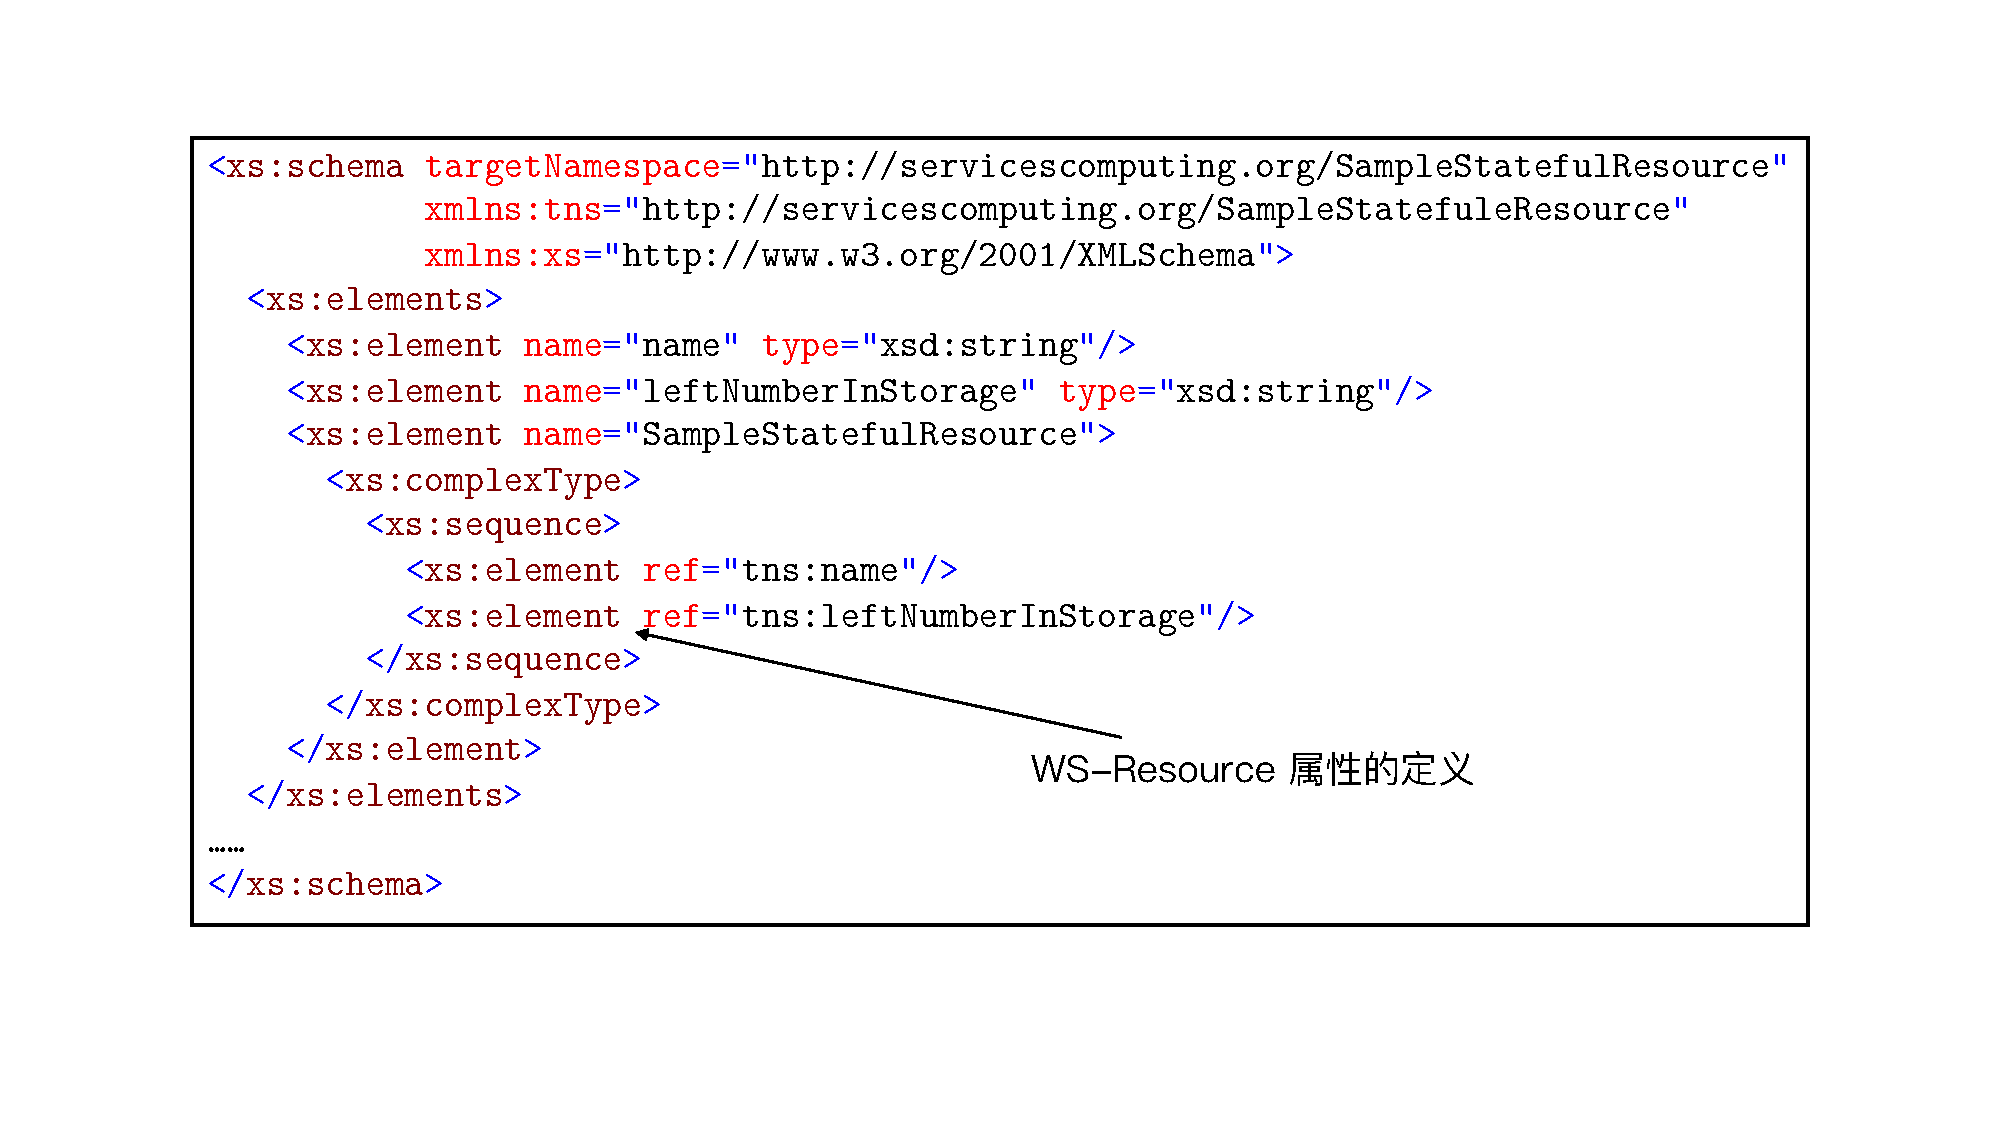
\includegraphics[width=0.79\textwidth]{images/状态资源的定义.pdf}
    \vspace{-1em}
\end{figure}

\paragraph*{资源定义的引入}~{} \par
\begin{figure}[H]
    \vspace{-0.5em}
	\centering
	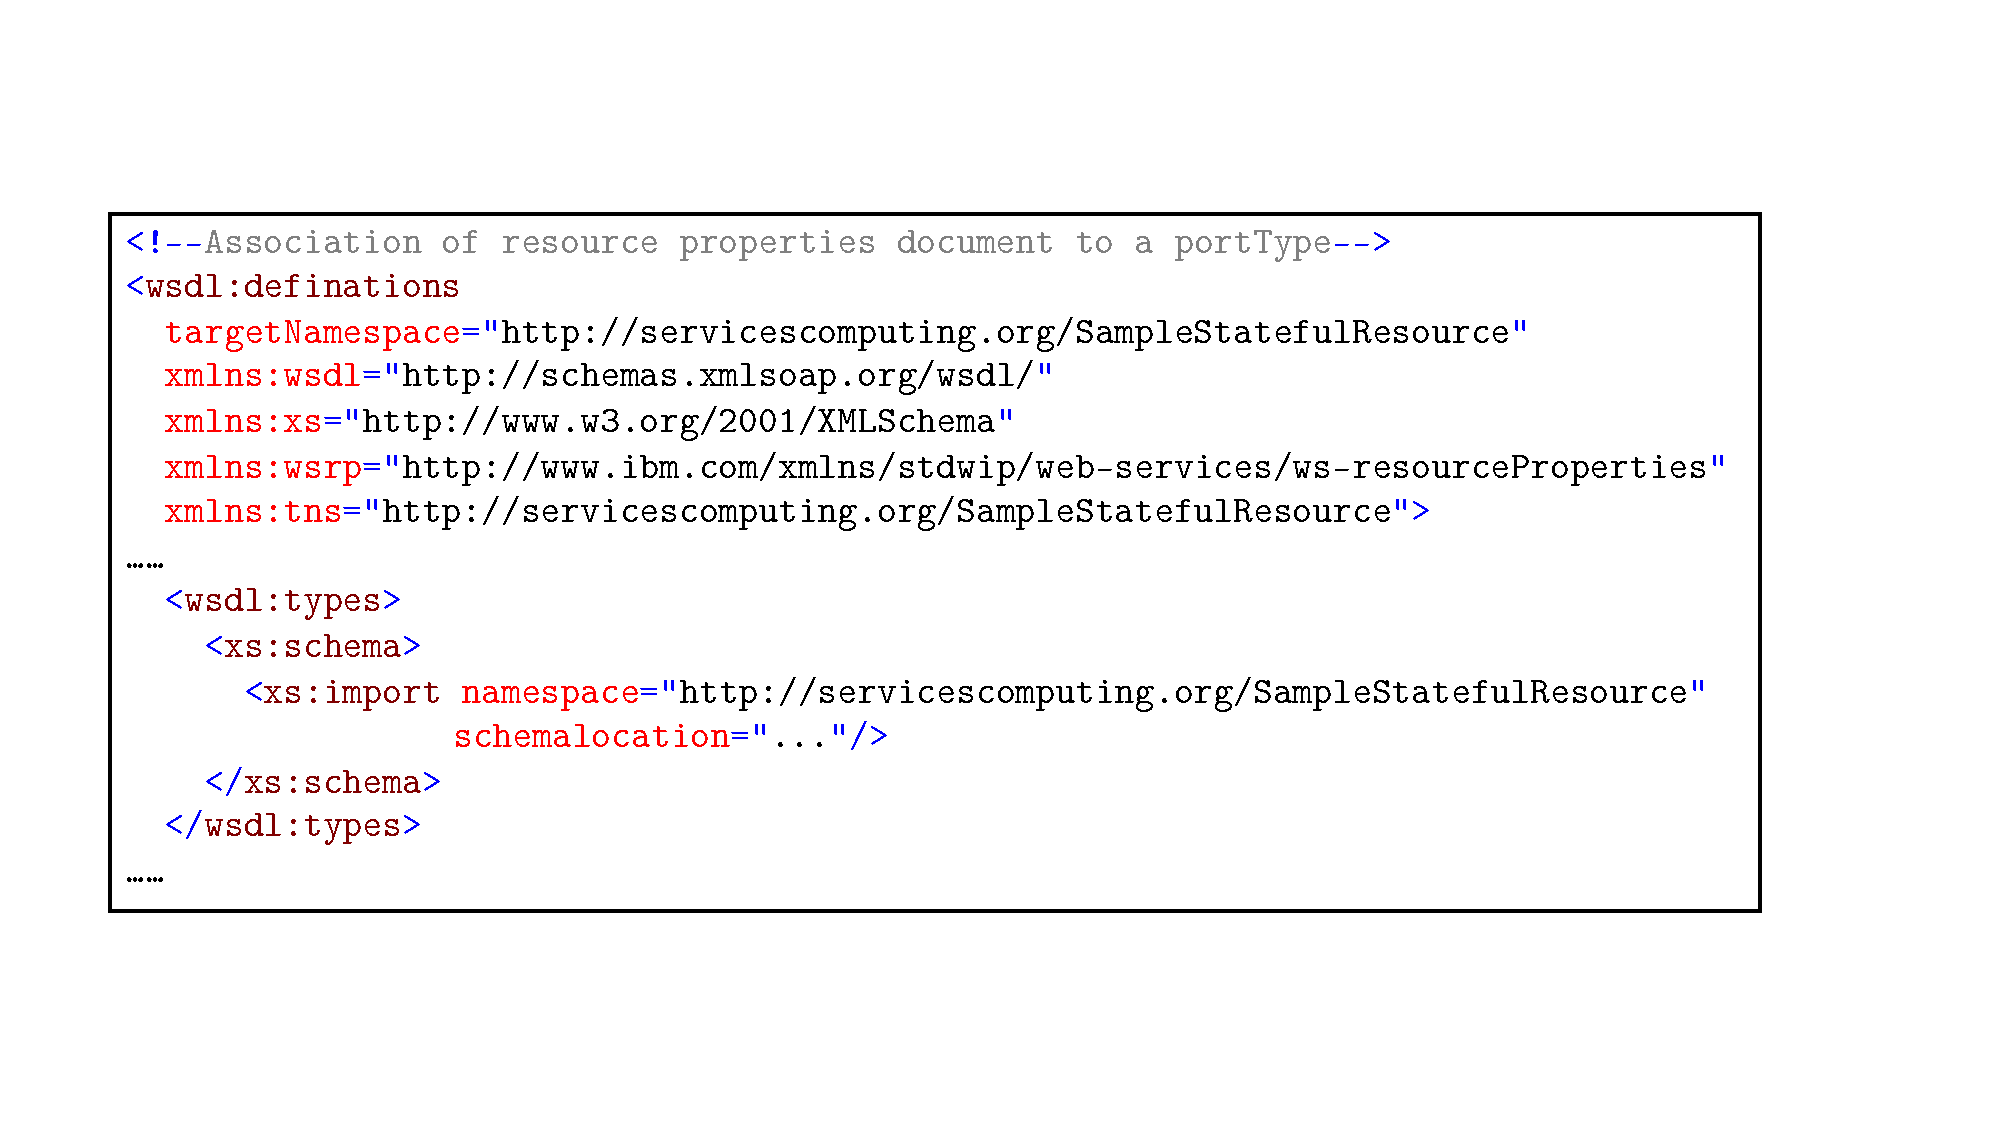
\includegraphics[width=0.79\textwidth]{images/资源定义的引入.pdf}
    \vspace{-1em}
\end{figure}

\paragraph*{将WS-Resource属性与接口进行关联}~{} \par
\begin{figure}[H]
    \vspace{-0.5em}
	\centering
	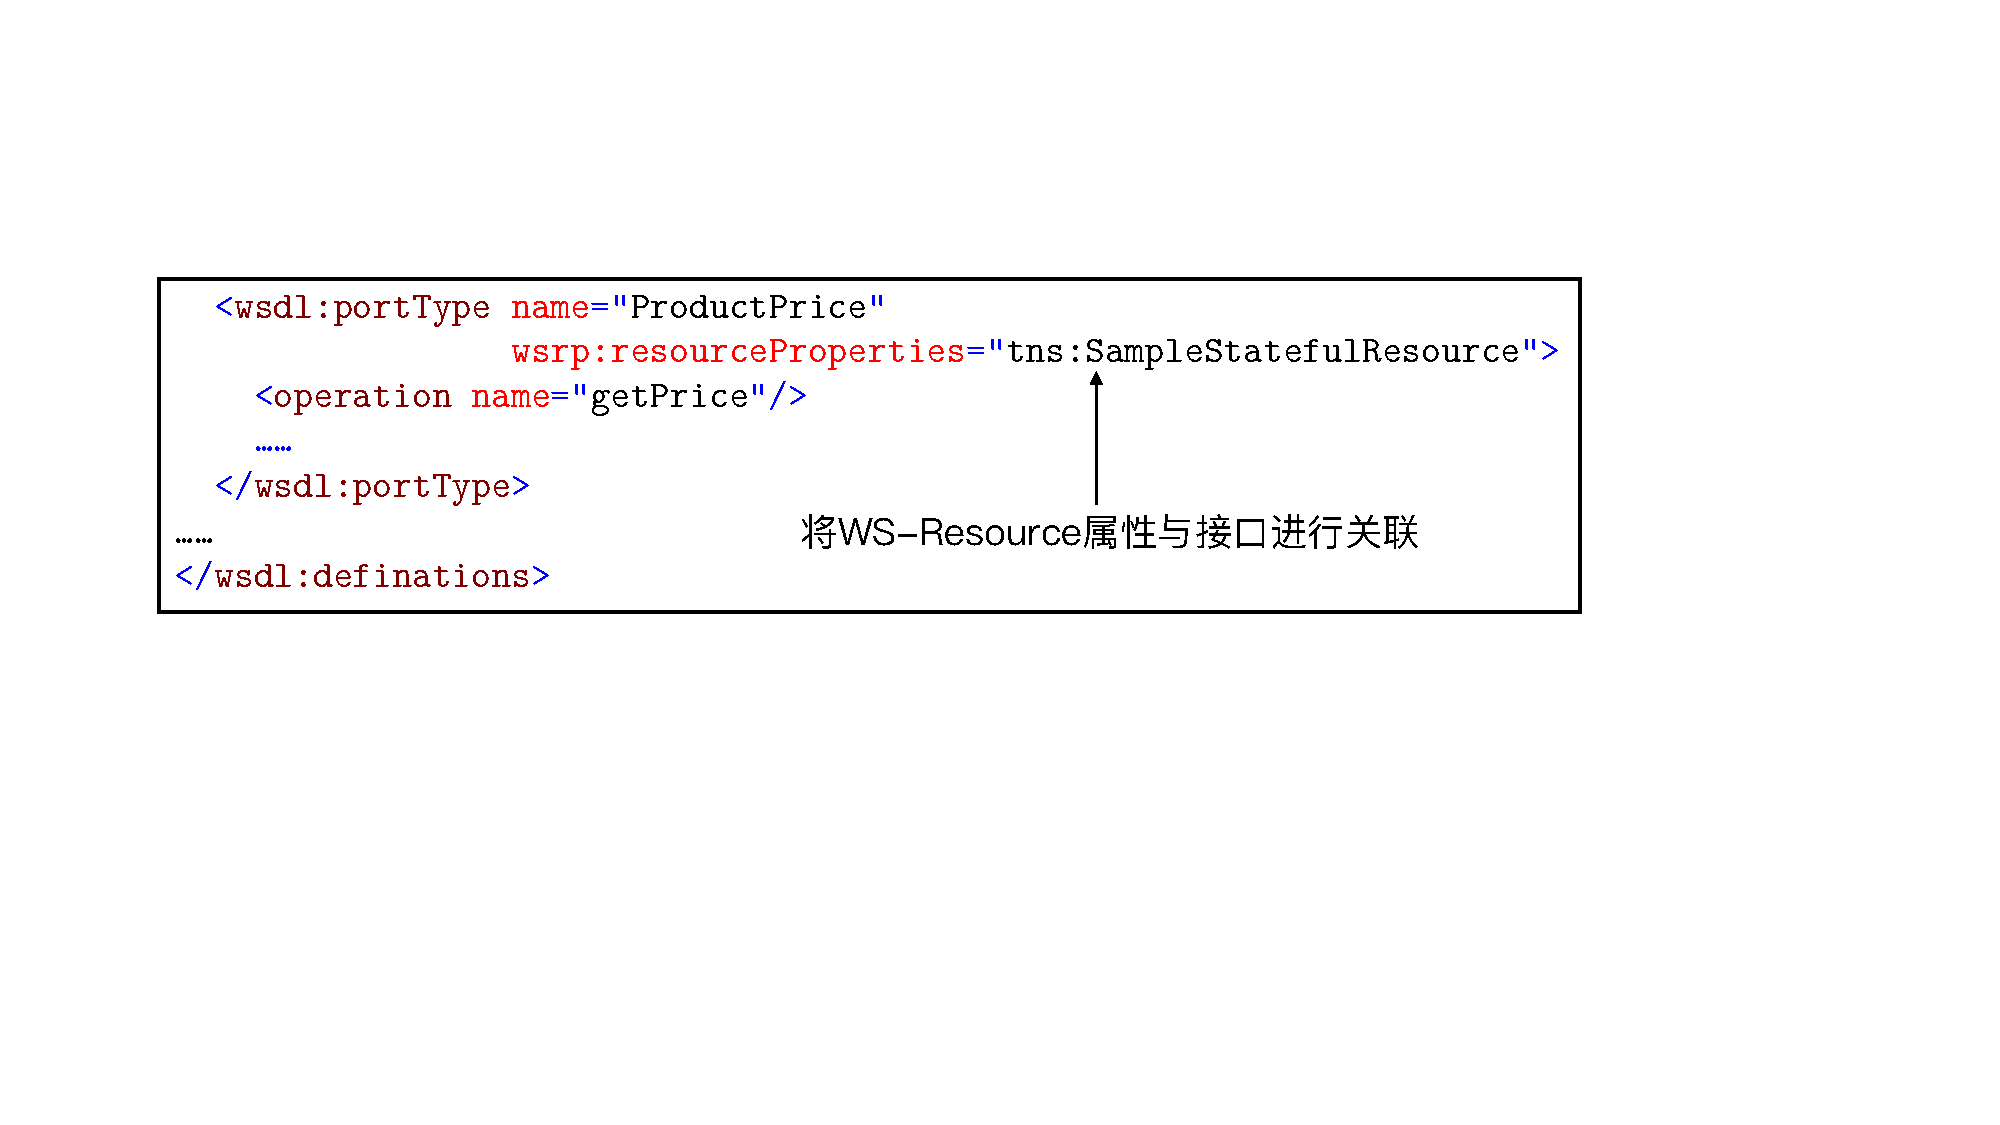
\includegraphics[width=0.75\textwidth]{images/将WS-Resource属性与接口进行关联.pdf}
    \vspace{-1.5em}
\end{figure}

\subsection{WS-Security}
虽然在链路与链路中间通过授权机制和HTTPS等等加密网络传输协议,确保在传输途中不会被篡改、不会被泄密,但由于整个 Web Service 是基于 XML,XML 是基于文本的明文,导致中间节点也可以看到并且去篡改消息。

\begin{wraptable}{r}{0.47\textwidth}
    \centering
    \vspace{-3.5em}
    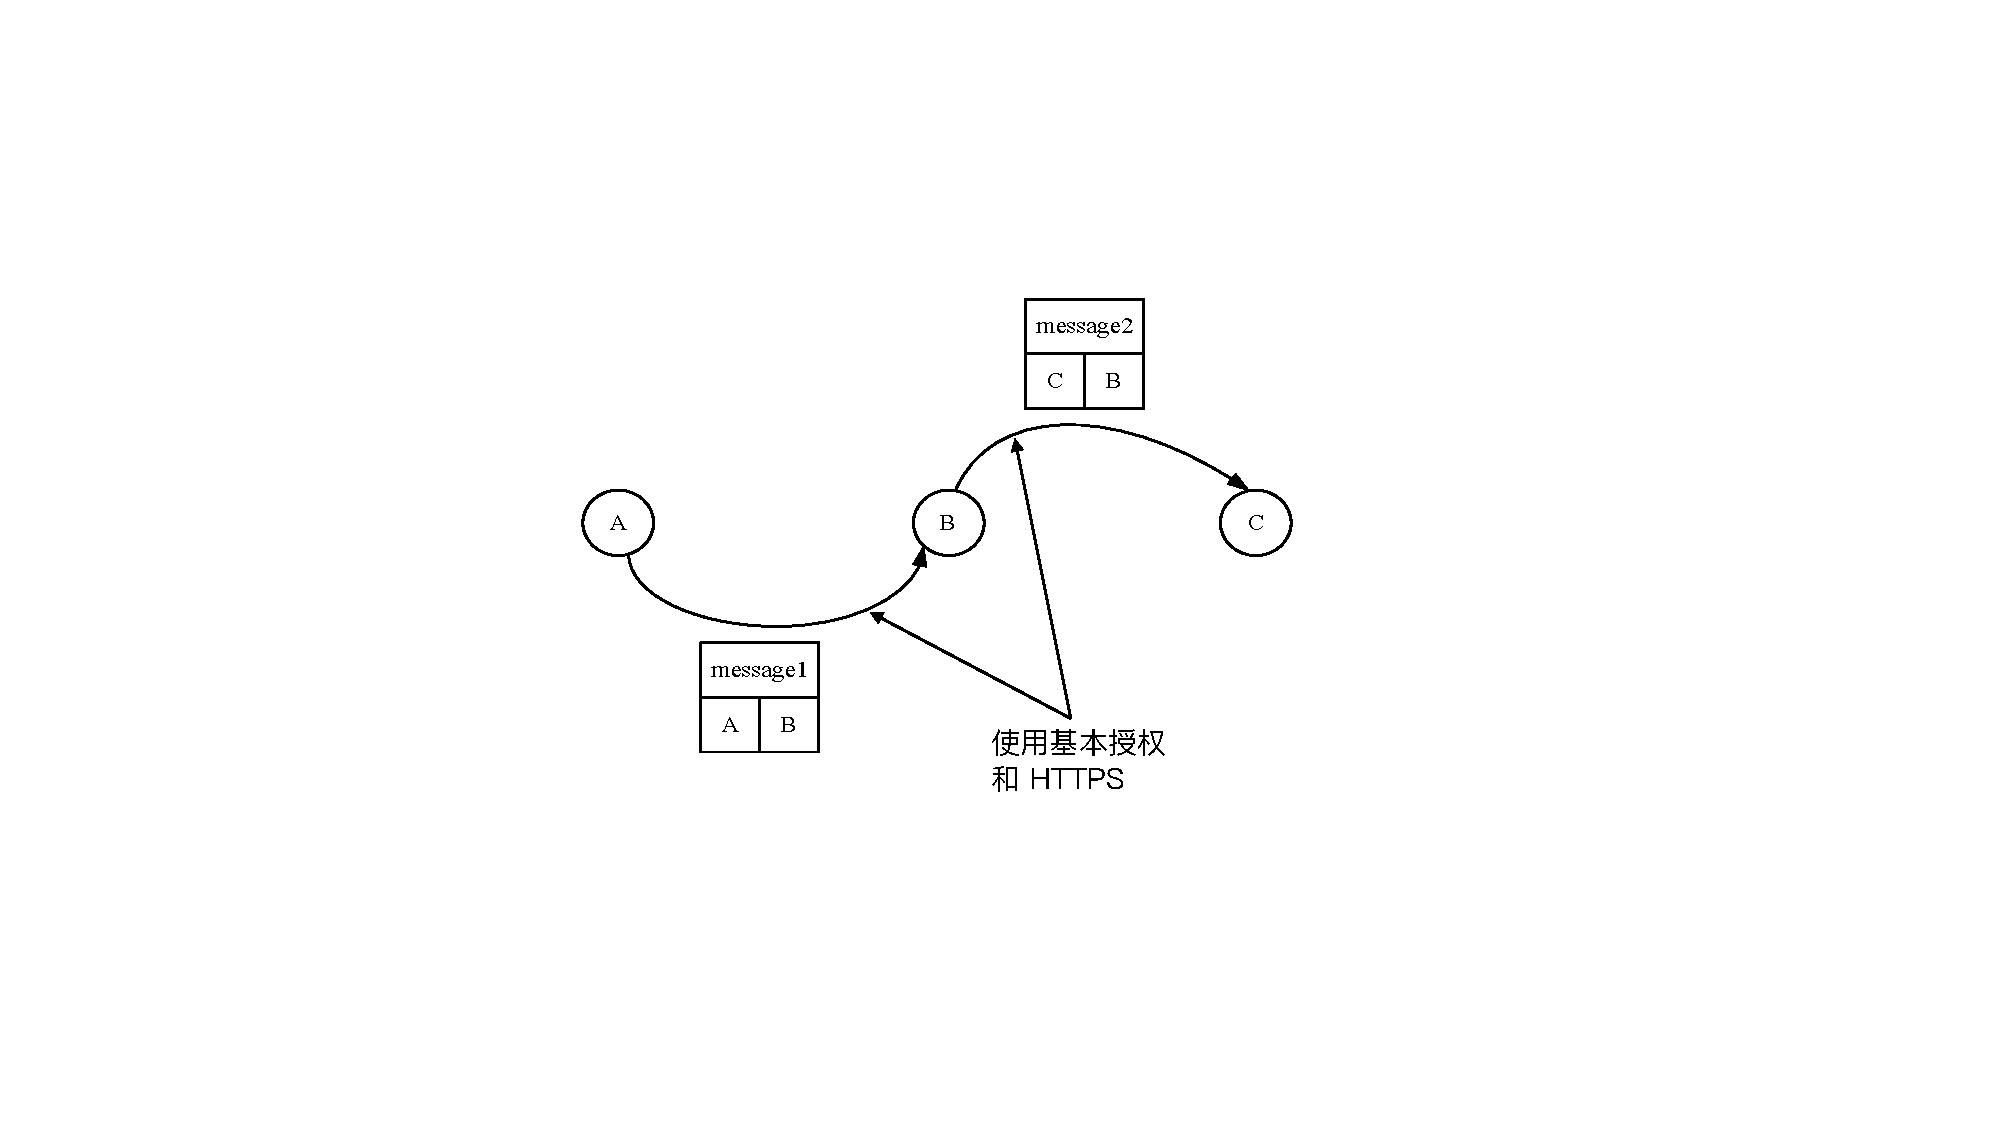
\includegraphics[width=0.45\textwidth]{images/使用基本授权和HTTPS.pdf}
    \vspace{-1.5em}
\end{wraptable}
WS-Security提供一组机制来帮助 Web 服务开发人员保护 SOAP 消息交换的安全。它是一组协议,增强了消息传递技术,解决了有关 Web 服务保护质量的三个基本问题:
\begin{itemize}
    \item 用户的身份验证和授权
    \item 消息完整性
    \item 消息加密
\end{itemize}

\subsubsection{WS-Security路线图}
\begin{figure}[H]
    \vspace{-0.5em}
	\centering
	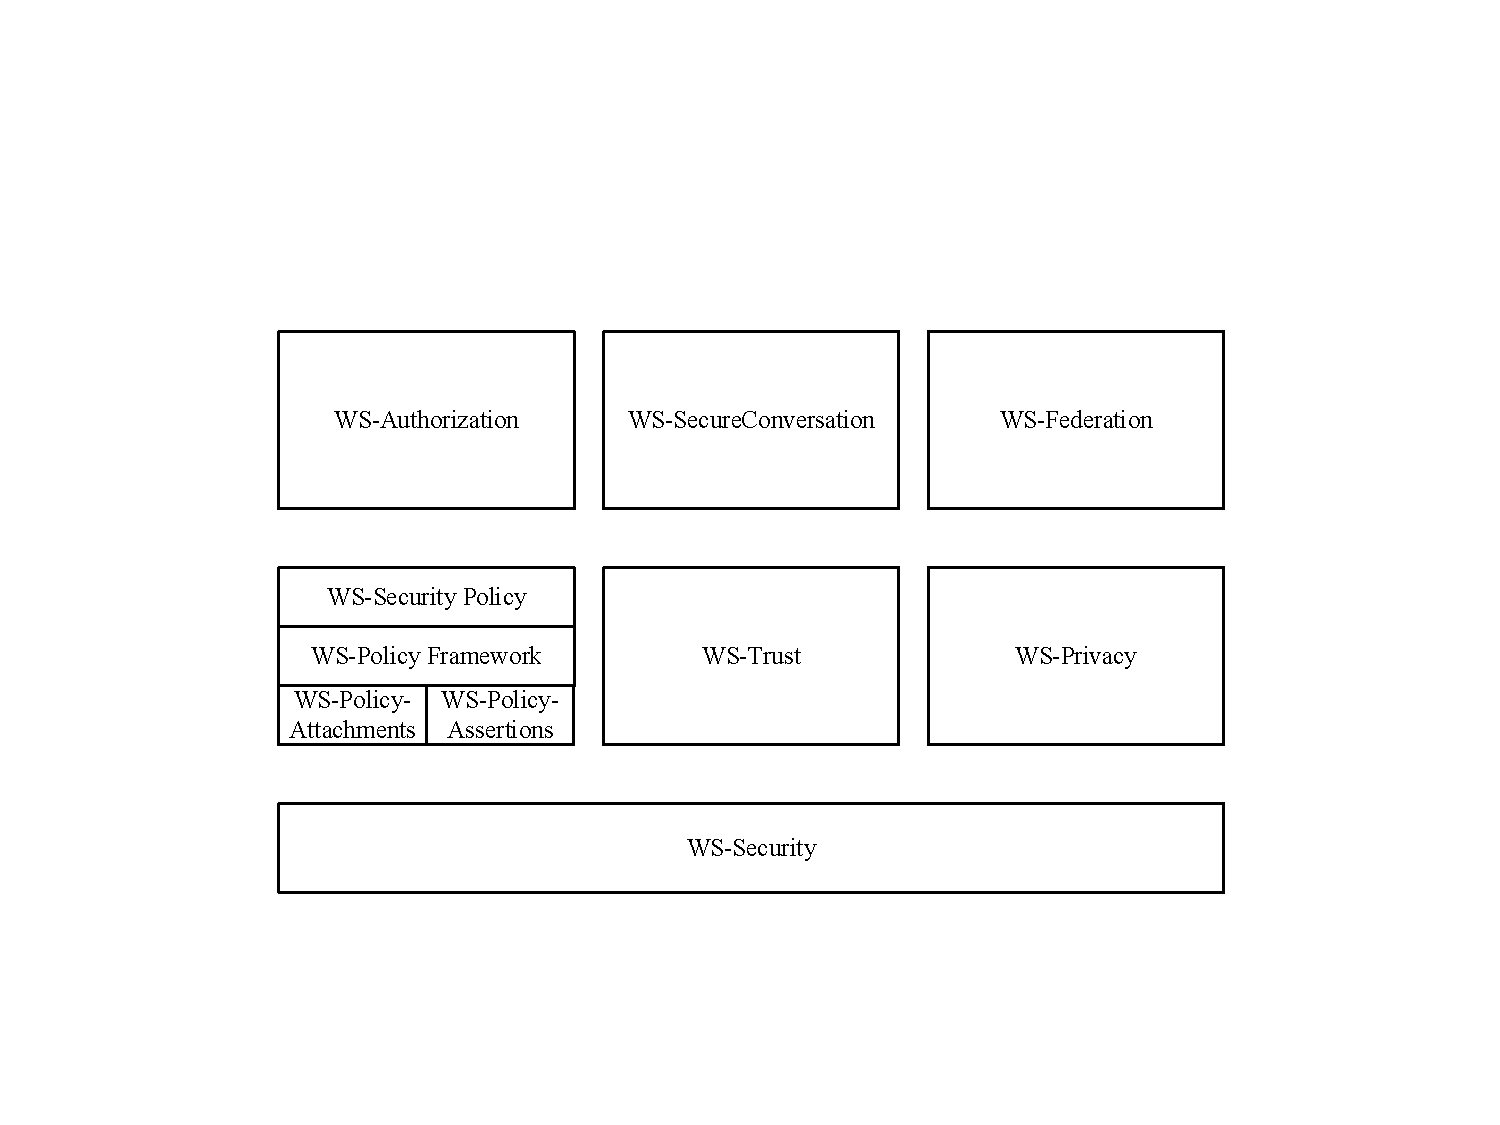
\includegraphics[width=0.75\textwidth]{images/WS-Security路线图.pdf}
    \vspace{-1.5em}
\end{figure}

\begin{itemize}
    \item WS-Policy提供了一种语法化的模型来指定Web服务端点策略,并通过包含WS-Security Policy进一步优化
    \begin{itemize}
        \item WS-Security Policy定义了一种语法,用于表达Web服务策略,它是一种语言,支持WS-Security规范
        \item WS-Policy Framework被定义为允许扩展来表达不仅限于安全策略的通用策略,它旨在在一致的Web服务框架内容纳特定领域策略语言的表达
        \item WS-Policy-Attachment提供了一种在Web服务中公布策略的方式,它建立在现有的WSDL和UDDI规范基础上,还支持可扩展性
        \item WS-Policy-Assertions语言提供了通用策略表达式,定义了Web服务的通用策略断言集合
    \end{itemize}
    \item WS-Trust定义了请求和发行用于建立信任关系的安全令牌的方法
    \item WS-Privacy规范描述了一种在WS-Policy描述中表达隐私声明并将隐私声明与消息相关联的模型
    \item WS-Authorization定义了Web服务如何管理授权数据和策略
    \item WS-SecureConversation基于安全令牌定义了安全上下文,用于安全通信
    \item WS-Federation定义了在不同信任域之间启用身份、帐户、属性、认证和授权联合的机制
\end{itemize}

\subsubsection{引入WS-Security后的SOAP消息}
\begin{wraptable}{r}{0.61\textwidth}
    \centering
    \vspace{-1.5em}
    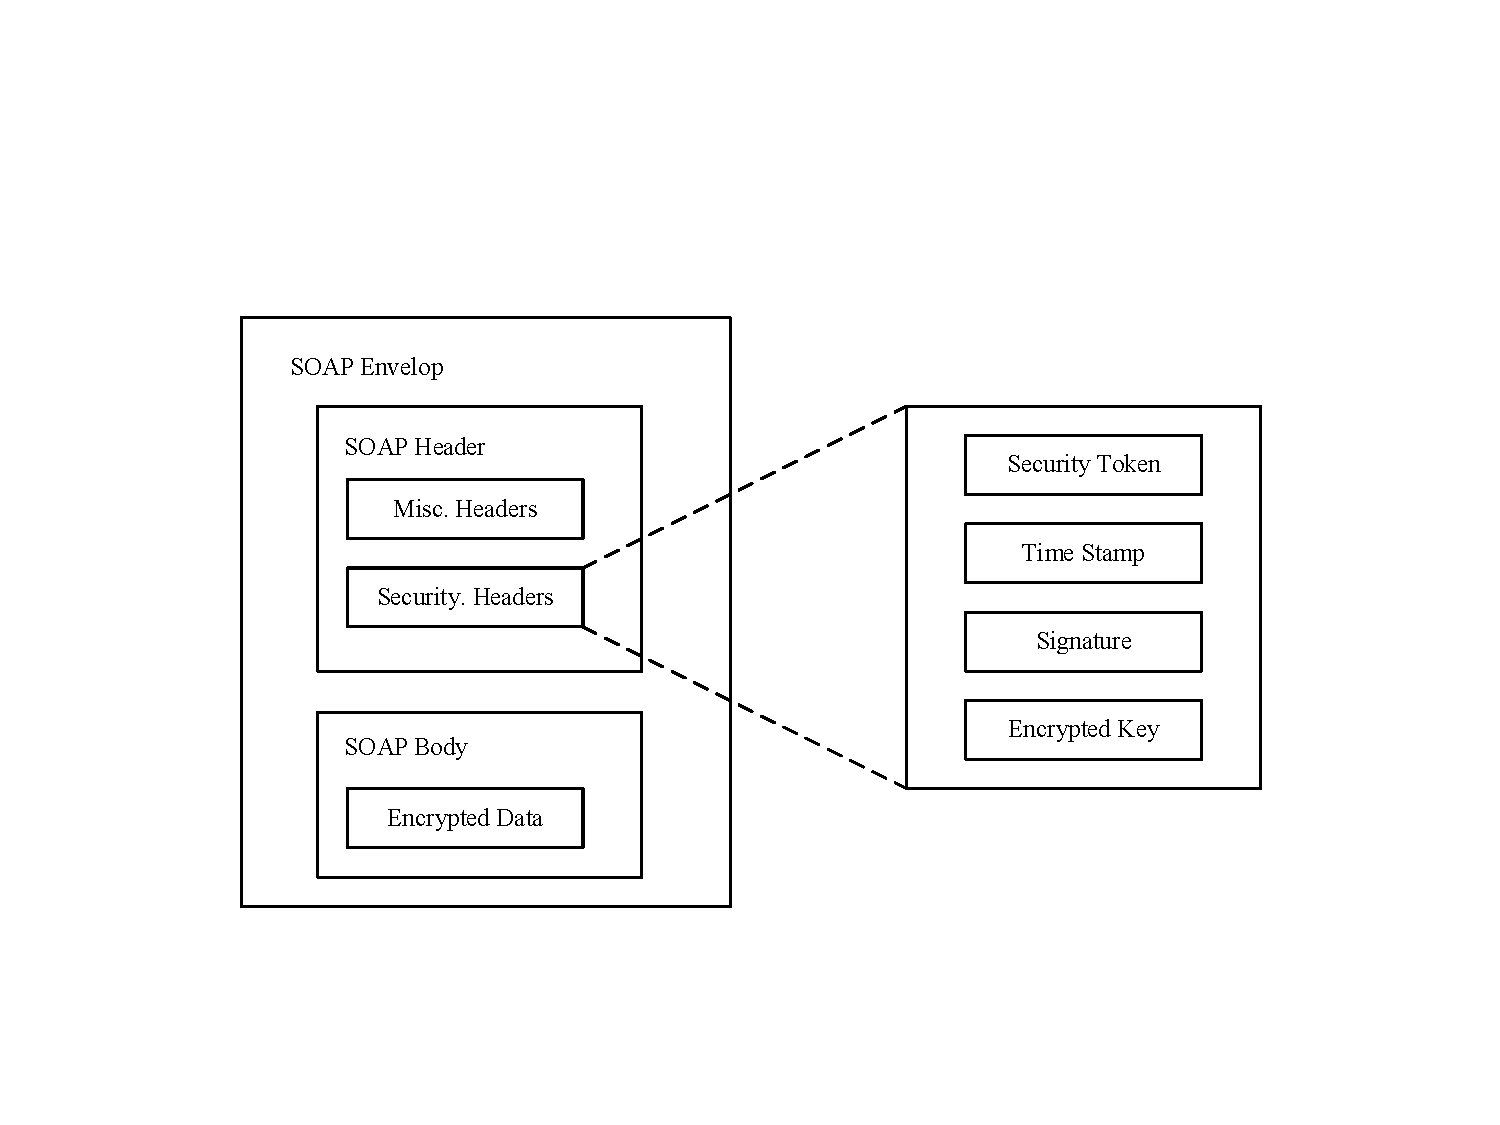
\includegraphics[width=0.6\textwidth]{images/WS-Security SOAP消息结构.pdf}
    \vspace{-1.5em}
\end{wraptable}
SOAP头部的添加:WS-Security通过添加SOAP头部来实现安全性。SOAP头部可以包含多个安全性相关的元素,如安全性令牌、签名和加密等。

SOAP正文的加密和签名:使用WS-Security可以对SOAP正文进行加密和签名。加密可以确保数据在传输过程中不被窃听或篡改,签名可以保证数据的完整性和真实性。

\paragraph*{加入身份验证的SOAP消息}~{} \par
\begin{figure}[H]
    \vspace{-0.5em}
	\centering
	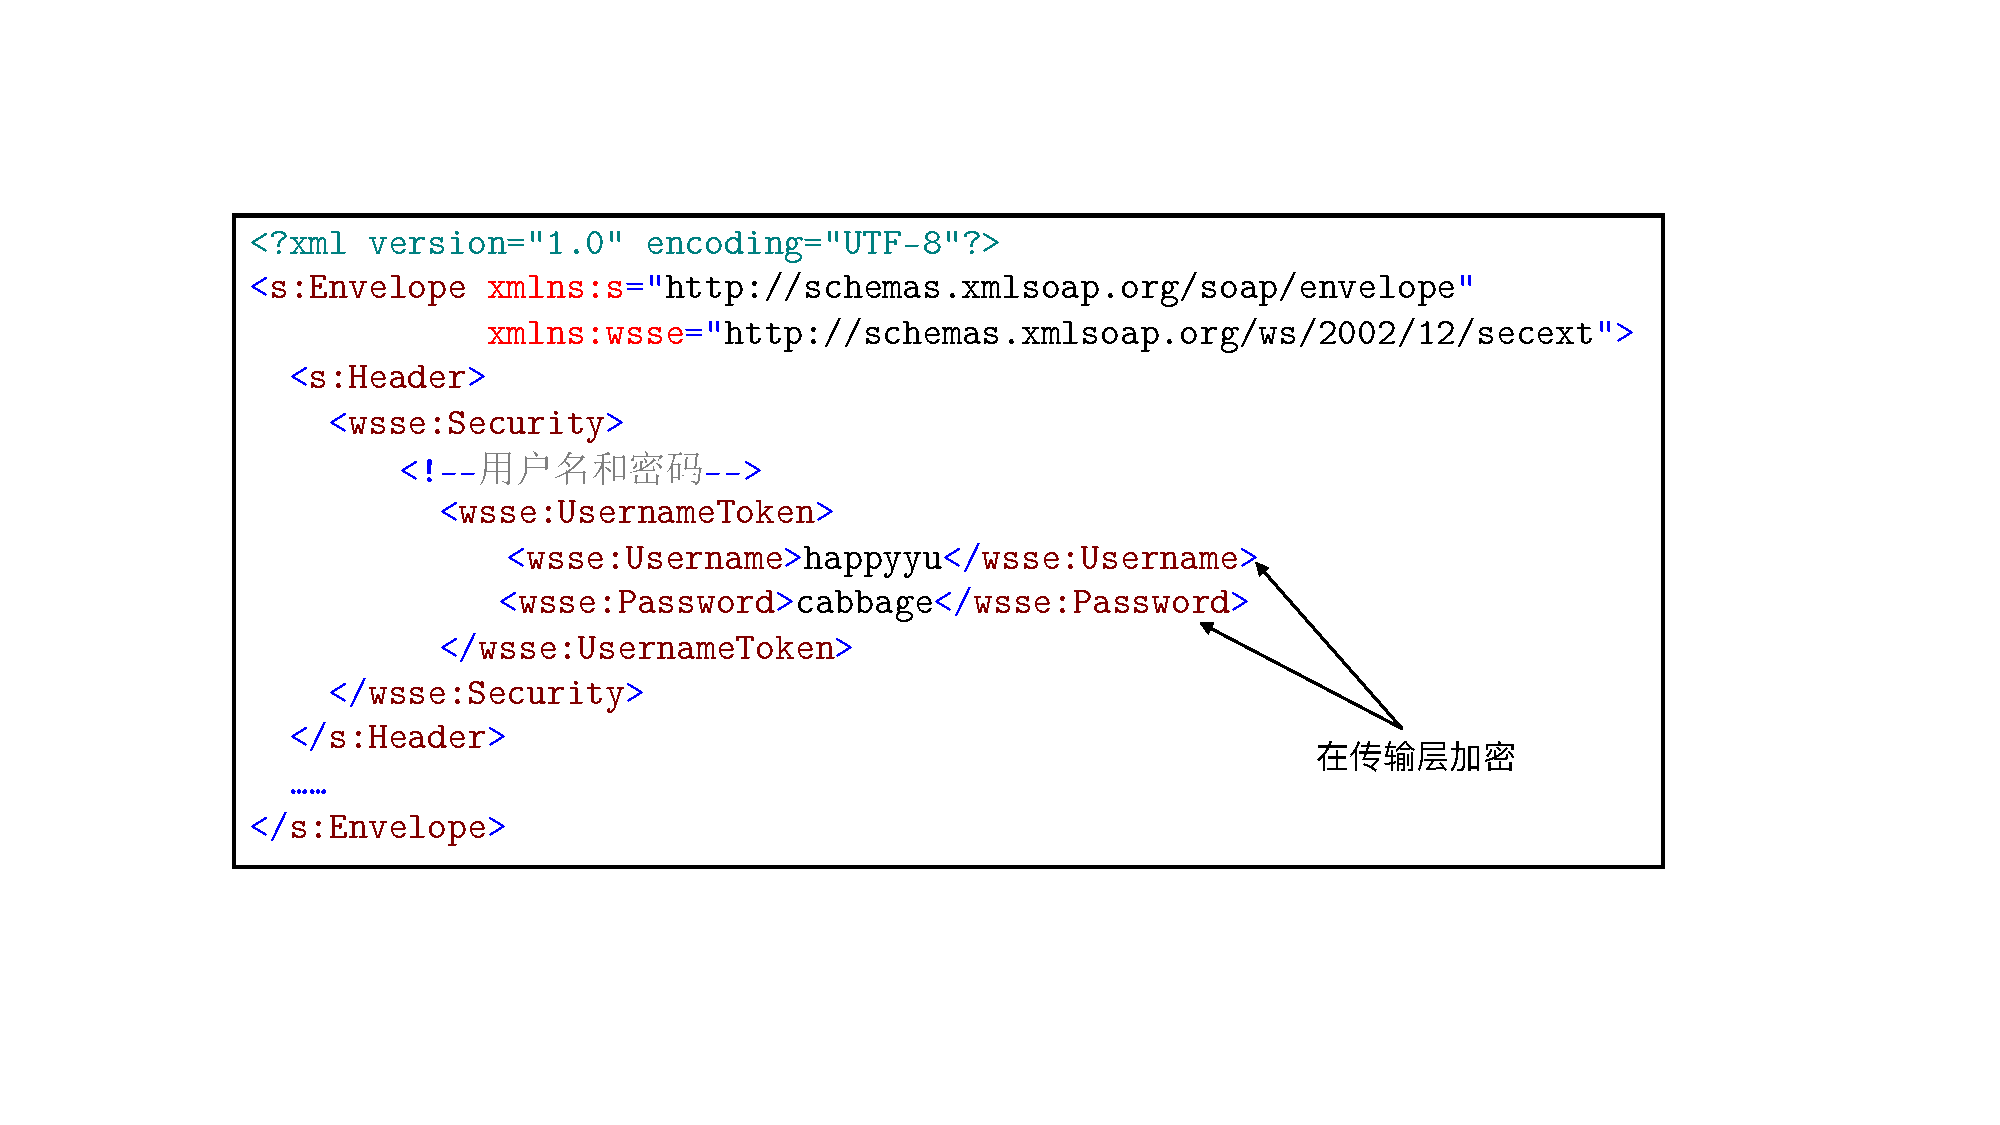
\includegraphics[width=0.85\textwidth]{images/加入身份验证的SOAP消息.pdf}
    \vspace{-1.5em}
\end{figure}

\paragraph*{加入数字签名的SOAP消息}~{} \par
\begin{figure}[H]
    \vspace{-0.5em}
	\centering
	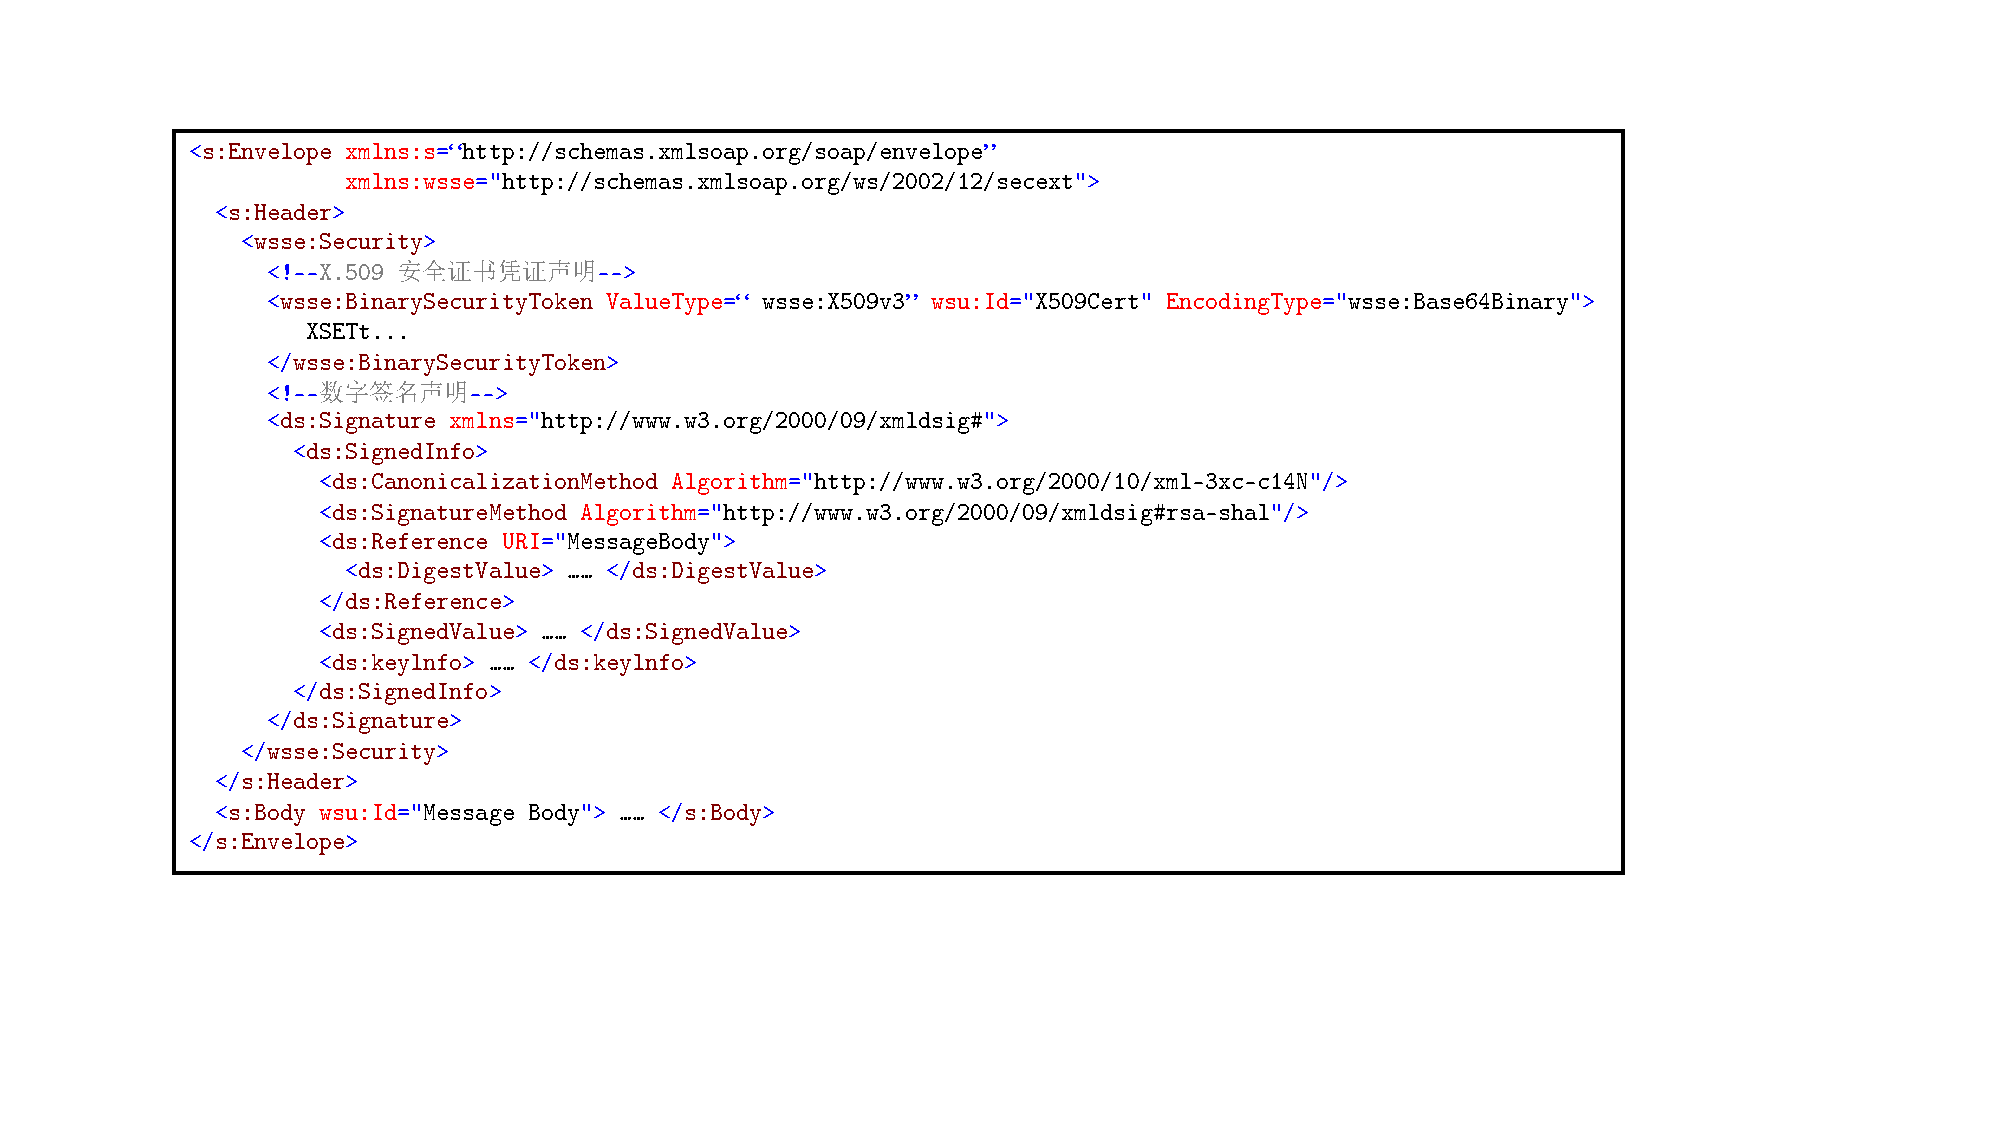
\includegraphics[width=\textwidth]{images/加入数字签名的SOAP消息.pdf}
    \vspace{-3em}
\end{figure}

\paragraph*{加入安全证书的SOAP消息}~{} \par
\begin{figure}[H]
    \vspace{-0.5em}
	\centering
	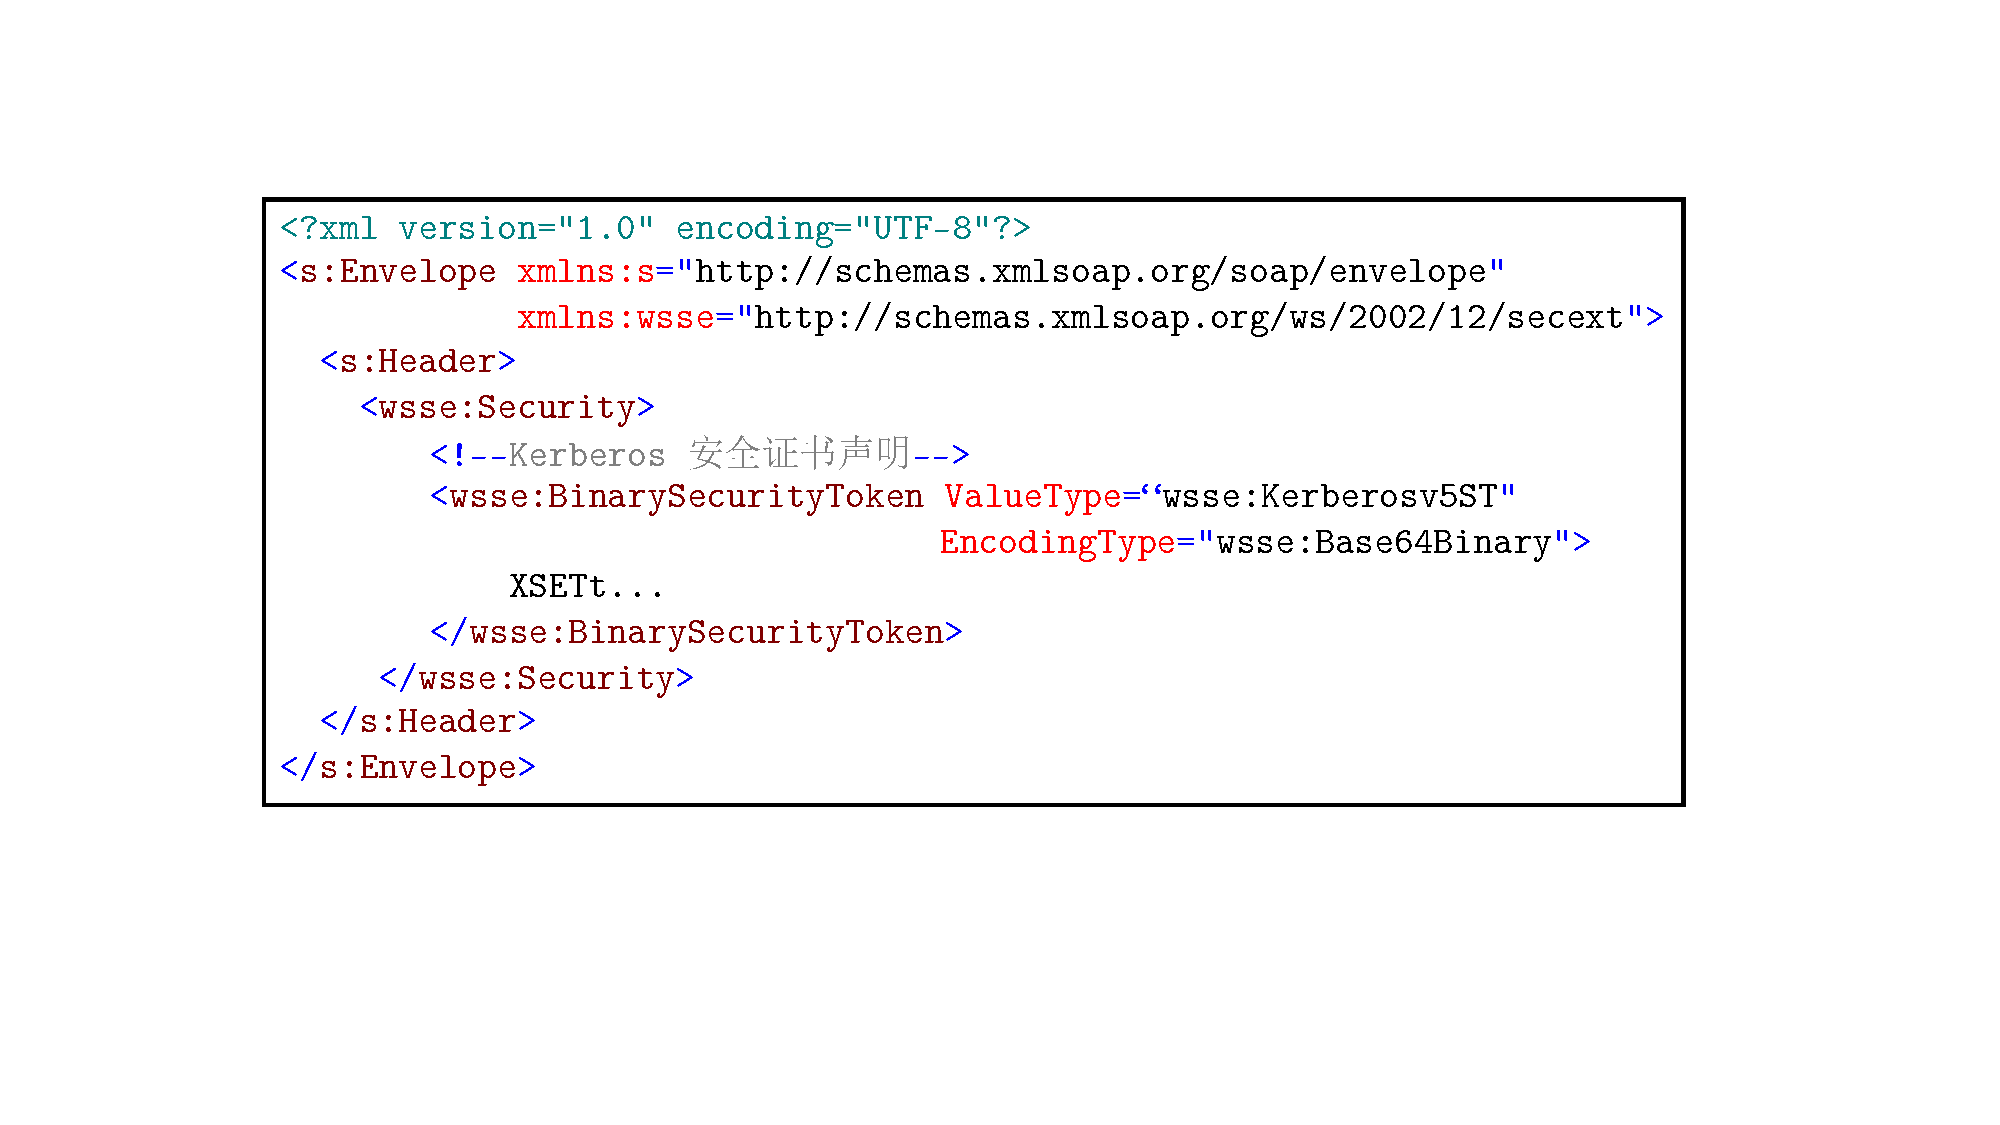
\includegraphics[width=0.75\textwidth]{images/加入安全证书的SOAP消息.pdf}
    \vspace{-1.5em}
\end{figure}

\paragraph*{加密的SOAP消息}~{} \par
\begin{figure}[H]
    \vspace{-0.5em}
	\centering
	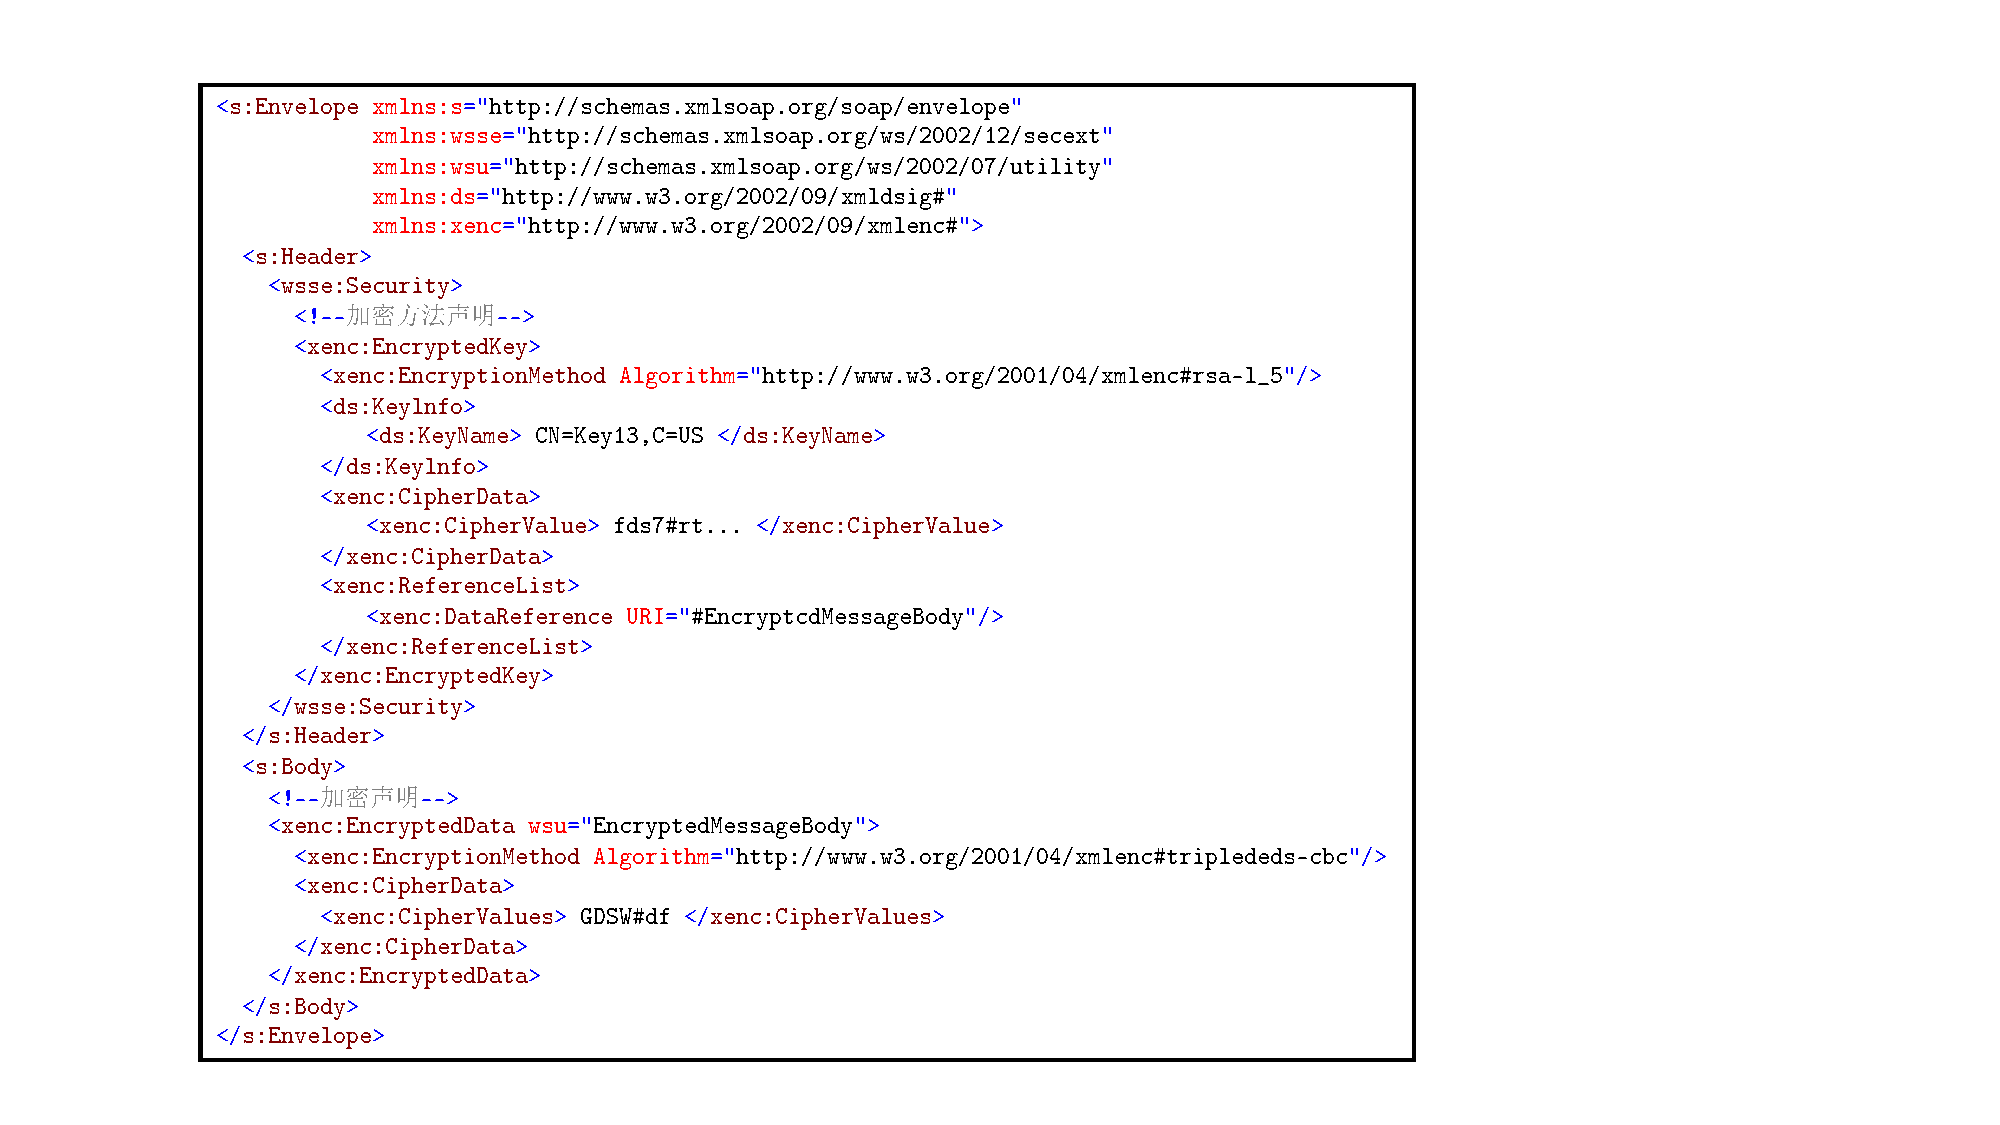
\includegraphics[width=0.95\textwidth]{images/加密的SOAP消息.pdf}
    \vspace{-1.5em}
\end{figure}


\subsection{WS-Coordination}
\begin{wraptable}{r}{0.68\textwidth}
    \centering
    \vspace{-2em}
    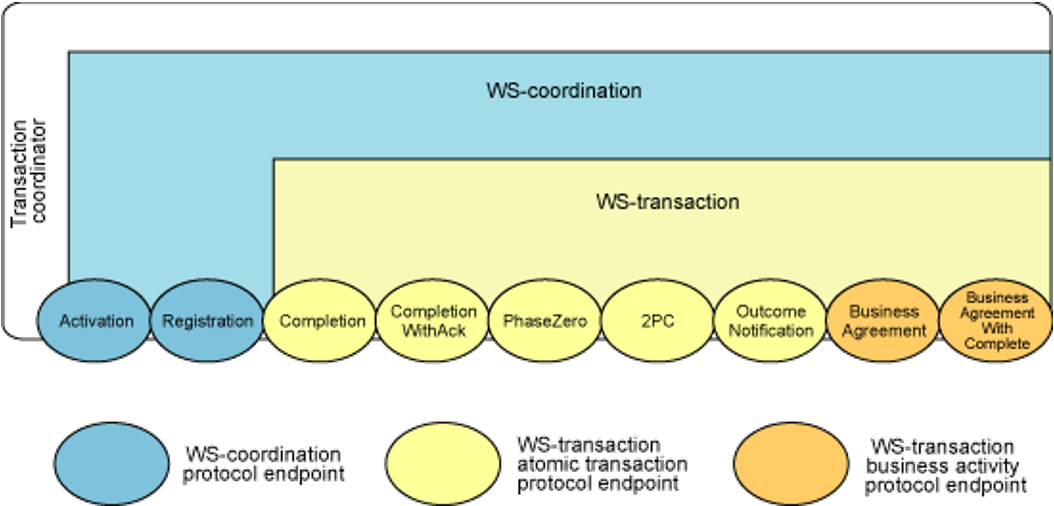
\includegraphics[width=0.68\textwidth]{images/WS-Coordination.png}
    \vspace{-8.5em}
\end{wraptable}
WS-Coordination 是用来发起、支持、完成多方参与、多消息的 Web Service 协作的通用机制,其定义了协调服务和协调上下文,是协调 Web Service 交互的框架

\subsubsection{协调框架}
\begin{itemize}
    \item 协调者服务提供了一个在 WSDL 中描述的服务,它具有启动协调任务、终止协调任务、允许参与者在任务中注册以及在一个组内生成协调上下文的能力
    \vspace{-0.8em}
    \begin{multicols}{2}
        \begin{itemize}
            \item 激活服务用于创建活动
            \item 注册服务用于协调协议选择和注册参与者
            \item 协调服务用于活动完成处理
        \end{itemize}
    \end{multicols}
    \vspace{-1em}
    \item 它还包括一个在 WSDL 中的接口,其他参与服务可以使用它来接收协调任务的结果通知
\end{itemize}

\subsubsection{协调上下文}
协调上下文支持Web服务在对话期间交换的所有消息。它包含一个指向协调服务的WS-Addressing端点引用,而该协调服务又包含用于识别正在协调的特定任务的信息。

\subsubsection{协调过程}
\begin{figure}[H]
    \vspace{-0.5em}
	\centering
	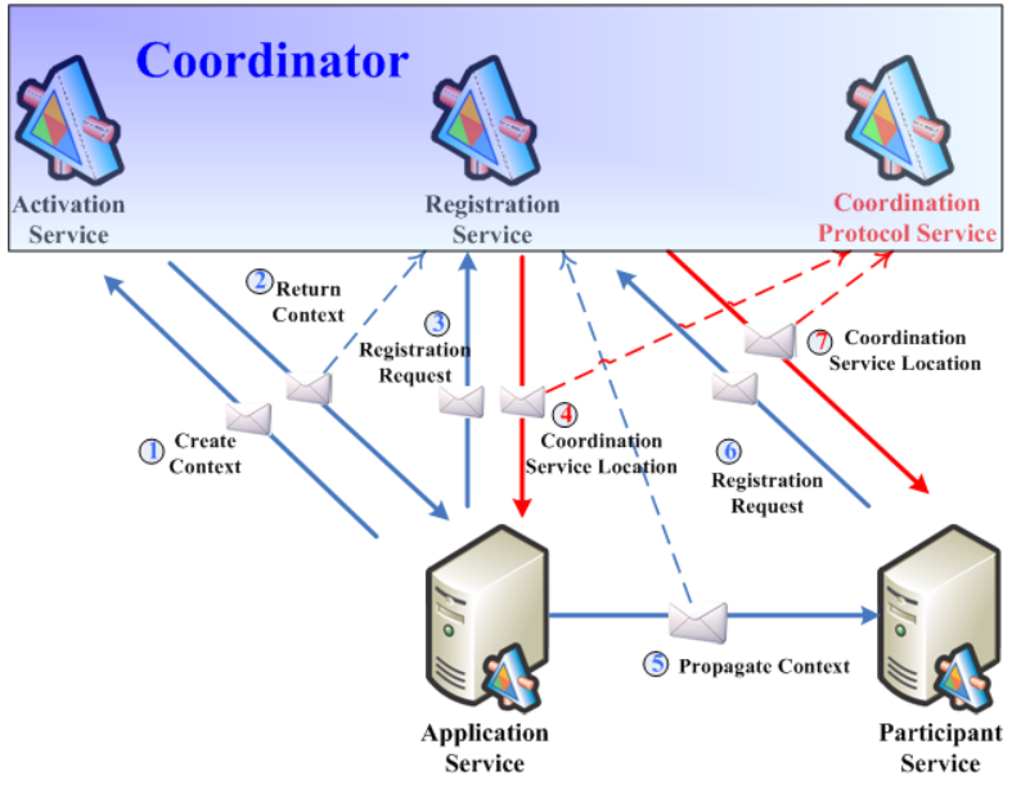
\includegraphics[width=0.7\textwidth]{images/协调过程.png}
    \vspace{-1.5em}
\end{figure}

\subsubsection{协调类型}
原子事务(AT)用于协调短期内在有限信任域内执行的活动。其定义一组要么全部成功要么全部失败的操作集合,保证数据的一致性。
\begin{figure}[H]
    \vspace{-0.5em}
	\centering
	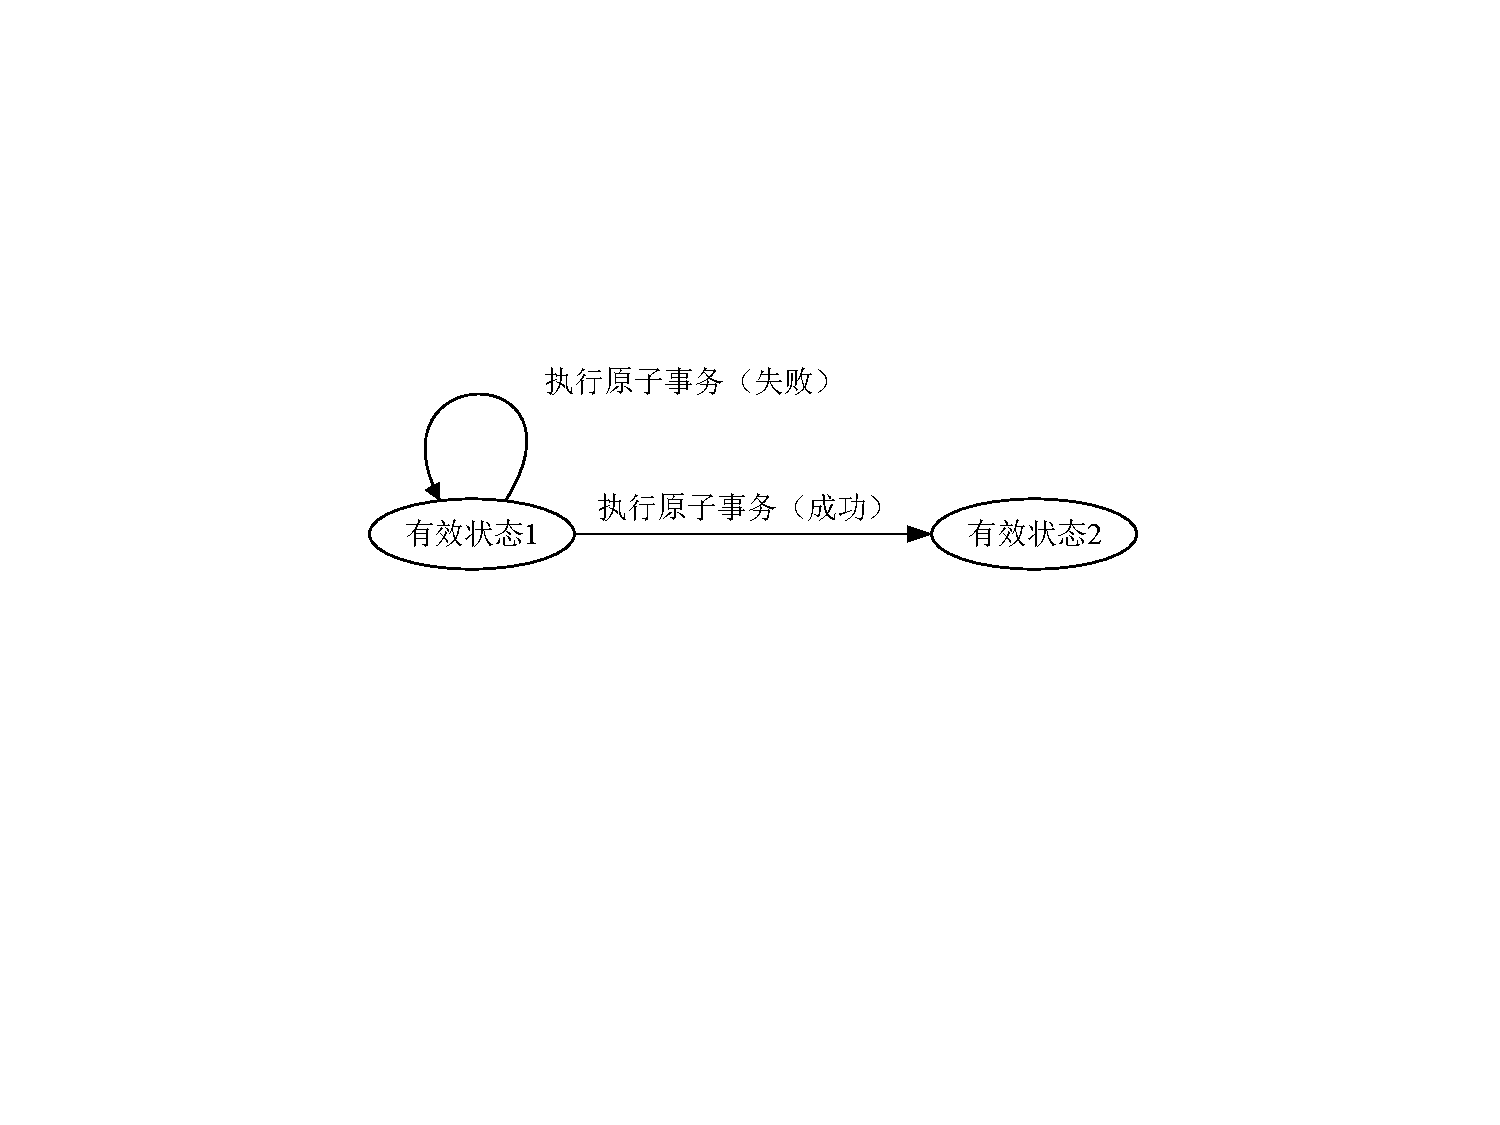
\includegraphics[width=0.45\textwidth]{images/WSAT.pdf}
    \vspace{-1.5em}
\end{figure}

业务活动(BA)用于协调长期执行且希望应用业务逻辑处理业务异常的活动。其定义一组关联的业务操作,在一组操作中存在一定的关联性,需要进行协调。
\begin{figure}[H]
    \vspace{-0.5em}
	\centering
	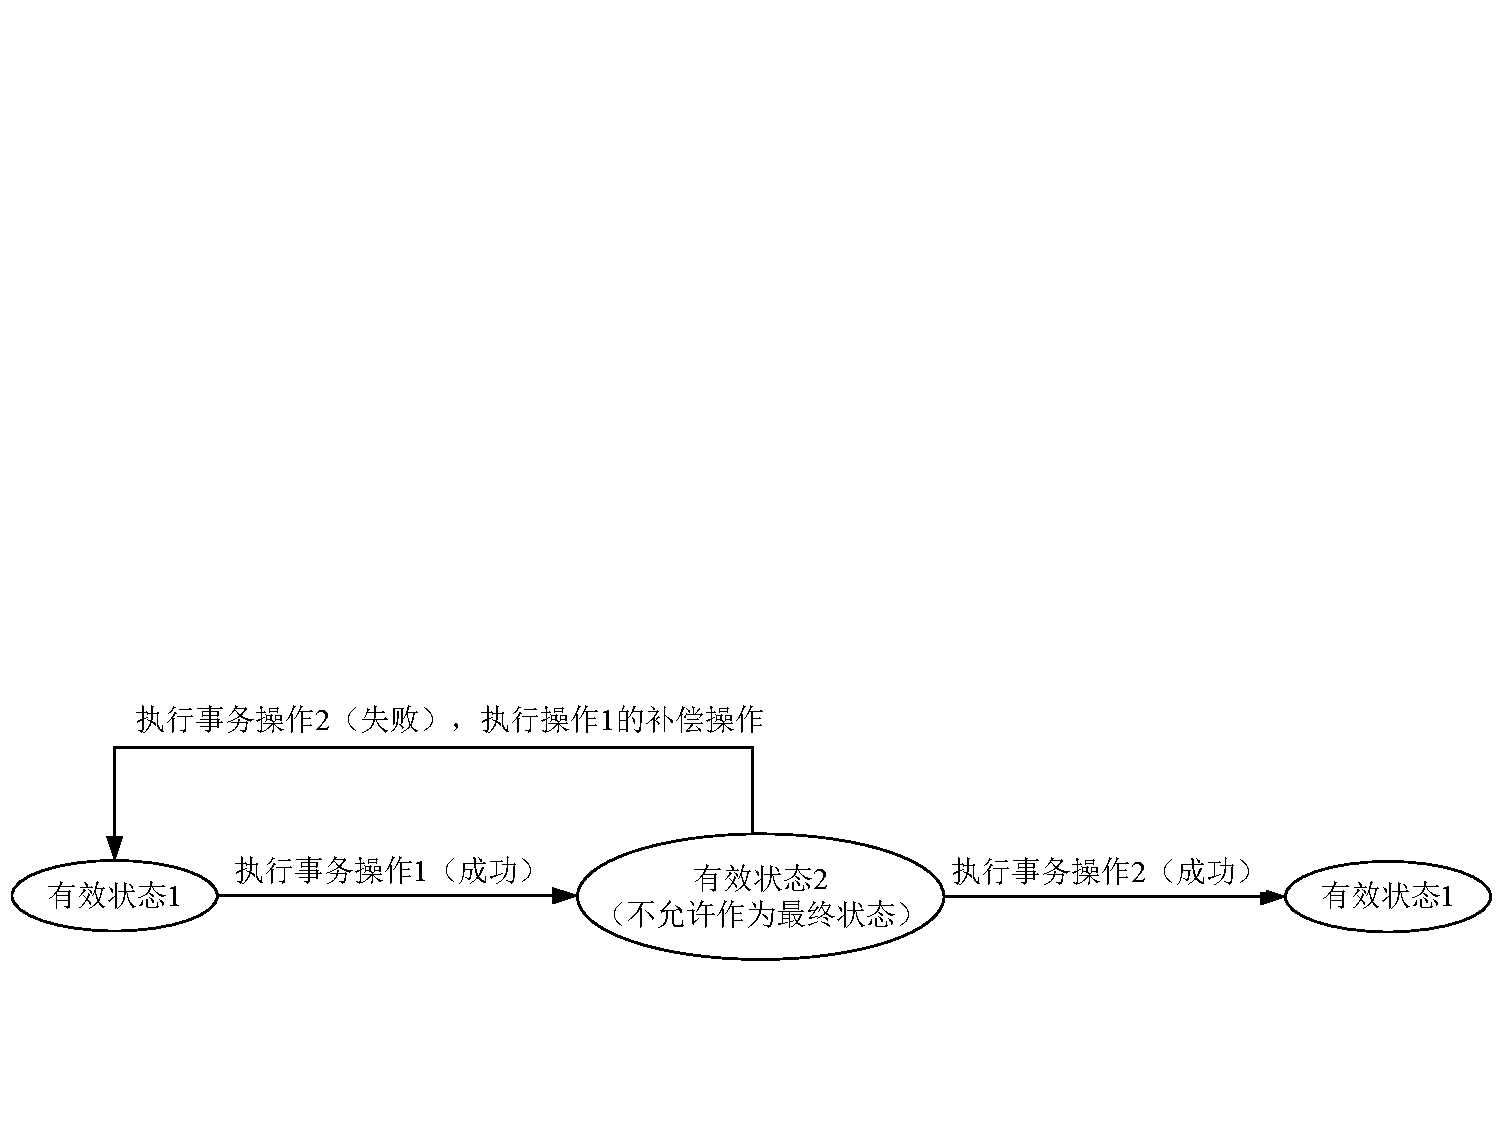
\includegraphics[width=0.8\textwidth]{images/WSBA.pdf}
    \vspace{-1.5em}
\end{figure}

\subsubsection{WSAT}
WSAT定义了短时的ACID事务:
\begin{itemize}
    \item 原子性(Atomicity):如果成功,则所有操作都发生,如果失败,则所有操作都不发生
    \item 一致性(Consistency):应用程序在完成时执行有效的状态转换
    \item 隔离性(Isolation):操作的效果在事务完成之前不会在事务之外共享
    \item 持久性(Durability):一旦事务成功完成,更改将在故障中幸存下来
\end{itemize}

它提供了用于WS-Coordination规范中描述的可扩展协调框架中使用的原子事务协调类型的定义

该规范为原子事务协调类型定义了特定的协议:
\vspace{-0.8em}
\begin{multicols}{3}
    \begin{itemize}
        \item Completion
        \item CompletionWithAck
        \item 2PC (Durable2PC)
        \item PhaseZero (Volatile2PC)
        \item OutcomeNotification
    \end{itemize}
\end{multicols}
\vspace{-1em}

\subsubsection{WSBA}
WSBA定义了长时间运行的业务交易,该规范定义了两种特定的协议来协调业务活动协调类型:
\begin{itemize}
    \item BusinessAgreementWithParticipantCompletion(参与者完成的业务协议)
    \item BusinessAgreementWithCoordinatorCompletion(协调者完成的业务协议)
\end{itemize}

开发人员可以在构建需要对长时间分布式活动结果达成一致的应用程序时使用任何或所有这些协议

\subsection{WS-Reliability}
\begin{itemize}
    \item WS-Reliability是一种基于SOAP的协议,旨在确保可靠的消息交换,包括:
    \vspace{-0.8em}
    \begin{multicols}{3}
        \begin{itemize}
            \item 保证交付
            \item 消息不会重复
            \item 确保消息顺序
        \end{itemize}
    \end{multicols}
    \vspace{-1em}
    \item WS-Reliability被定义为SOAP头扩展,通过故障代码扩展SOAP故障规范以指定可靠性消息特定的故障值
    \item 在实现可靠消息传递的模型中,发送方向接收方直接发送带有全局唯一标识符的SOAP消息,并等待接收方发送回确认消息。如果发送方未收到确认消息,则会尝试重新发送SOAP消息
    \item 为了保证消息不会重复和顺序正确,可以使用SOAP消息中的标识符来去重和重排序消息
\end{itemize}

